\documentclass[article,oneside]{memoir}
\usepackage[T1]{fontenc}
\usepackage{mathptmx,upquote,alltt}
\IfFileExists{helvet.sty}{\usepackage[scaled=0.92]{helvet}}{\relax}
\IfFileExists{couriers.sty}{\usepackage[scaled=0.95]{couriers}}{\relax}
\usepackage{float,graphicx,xspace,framed,xcolor}
\definecolor{shadecolor}{rgb}{0.97,0.97,0.97}
\definecolor{lightblue}{rgb}{0.93,0.95,1.0}
\definecolor{darkblue}{rgb}{0,0,0.6}
\definecolor{darkred}{rgb}{0.6,0,0}
\setlength{\parindent}{0pt}
\nonzeroparskip
\usepackage[
   bookmarks=true,
   hyperindex = true,
   pdfpagemode = useoutlines,
   pdfpagelabels = true,
   plainpages = false,
   colorlinks = true,
   linkcolor=darkblue,
   filecolor=darkblue,
   citecolor=darkblue,
   urlcolor=darkblue,
]{hyperref}
\usepackage{attachfile}
\usepackage{memhfixc}
\raggedbottom
\hyphenation{StatRep}
\chapterstyle{article}
\DeclareTextFontCommand{\Code}{\ttfamily}
\newcommand*{\StatRep}{\textsf{StatRep}\xspace}
\newcolumntype{P}[1]{>{\raggedright\arraybackslash}p{#1}}
\setlength{\FrameSep}{1pt}
\title{The \StatRep User's Guide}
\author{Tim Arnold and Warren F. Kuhfeld\\SAS Institute Inc.}
\makeindex
\begin{document}
\maketitle
\tableofcontents*%\listoftables\listoffigures
%%%%%%%%%%%%%%%%%%%%%%%%%%%%%%%%%%%%%%%%%%%%%%%%%%%%%%%%%%%%%%%%%%%
%%%%%%%%%%%%%%%%%%%%%%%%%%%%%%%%%%%%%%%%%%%%%%%%%%%%%%%%%%%%%%%%%%%
\chapter{Synopsis}
The \StatRep system consists of a \LaTeX\ package and a suite of SAS macros that
support SAS users who want to create documents with reproducible results.

The \LaTeX\ package provides two environments and
two tags that work together to display your SAS code and results and to
generate the SAS program that produces those results. The two environments
(\Code{Datastep} and \Code{Sascode}) display SAS code.
The two tags (\cs{Listing} and \cs{Graphic}) display SAS output.

The generated SAS program includes calls to the \StatRep macros that use the SAS
Output Delivery System (ODS) document to capture the output as external files.
These SAS macros are included in the package file \Code{statrep\_macros.sas}.
The package is available at \url{http://support.sas.com/StatRepPackage}

Bundled with the StatRep package is the \Code{longfigure} package for
multipage figures.
%%%%%%%%%%%%%%%%%%%%%%%%%%%%%%%%%%%%%%%%%%%%%%%%%%%%%%%%%%%%%%%%%%%
%%%%%%%%%%%%%%%%%%%%%%%%%%%%%%%%%%%%%%%%%%%%%%%%%%%%%%%%%%%%%%%%%%%
\chapter{Introduction}

At the end of a research project, one of the most difficult tasks remains: documentation.
The task is especially difficult with computational research because you
must ensure that the displayed program code works as expected and exactly produces the
displayed output.

The \StatRep package, a single-source document system,
is an open-source software project that you can use for your own research documentation
to ensure that the results you display can easily be reproduced by your readers.
The \StatRep package is based on the \LaTeX\ typesetting system. You write your paper using
both the usual \LaTeX\ markup and the customizations and SAS macros that this package provides.
The system reads the code and markup from the single source (your document) and creates a
SAS program. This automatically generated SAS program produces the results that are displayed
in your document.

Comparable projects such as Sweave (Leisch 2002) and SASweave  (Lenth 2007)
address the problem of reproducibility through the use of a special intermediate language.
Although similar in spirit to those systems, \StatRep differs in that it is a
normal \LaTeX\ package; no special steps are needed to create the \LaTeX\
file or the SAS program.   In addition, \StatRep provides both a complete, customizable system for
automatic handling of multiple outputs and page breaking and an easy-to-use,
flexible method for output selection.

When you use the \StatRep \LaTeX\ package, you follow a four-step process to
create an executable document that enables you to create
reproducible research results:
\begin{enumerate}
\item Create your \LaTeX\ source file so that it contains your text, data, and SAS code.

\item Compile the document with pdf\LaTeX. You can use a LaTeX-aware
      editor such as \TeX works, or you can use the command-line command \Code{pdflatex}.
      This step generates the SAS program that is needed to produce the results.
      If the name of your document is \textit{myarticle.tex}, the name of the generated SAS
      program is \textit{myarticle\_SR.sas} by default.

\item Execute the SAS program to capture your output.

During execution of the SAS program, for each code block in your document,
SAS creates a SAS Output Delivery System (ODS) document that contains the resulting output.
For more information about ODS documents, see the
\textit{SAS Output Delivery System User's Guide}.
For each output request (the included \cs{Listing} and \cs{Graphic} tags) in your document, SAS replays the specified output objects
to external files. All of your requested output is generated and captured when you
execute the generated SAS program.

\item Recompile the document with pdfLaTeX. This step compiles your
      document to PDF, this time including the SAS results
      that are generated in the preceding step.

      In some cases listing outputs may not be framed properly after this step.
      If your listing outputs are not framed properly, repeat this step so that
      LaTeX can remeasure the listing outputs.

\end{enumerate}

When you need to make a change in your data or SAS code, you make the change in
one place (the \LaTeX\ source file) and repeat steps 2 through 4.
Your changes are automatically displayed in your code and in your results.
You perform the steps only as needed---when you change your data or code.

You can share your \LaTeX\ source with colleagues and be sure that your results
are reproducible. Any SAS user can reproduce your analysis with your \LaTeX\ document
and the supplemental files that are described in this manual.

\section{Requirements for the \StatRep Package}
\index{package!requirements}
To use the \StatRep package, you need SAS 9.2 or later,
the \LaTeX\ typesetting system
(the  pdf\LaTeX\ typesetting engine must be version 1.30 or later), and the \StatRep package itself.

For complete step-by-step instructions for installation, see section \ref{install}.
\section{Package Usage}
\index{package!usage}
  To use the \StatRep package, include it in your document preamble after you
  declare the \Code{documentclass}.
  Figure \ref{fig:usage} displays an example of how you can use the \StatRep package.

\begin{figure}[H]
\begin{shaded}
\begin{verbatim}
\documentclass{book}
\usepackage[figname=output,resetby=chapter]{statrep}
\end{verbatim}%
\end{shaded}
\caption{Example of Using the \StatRep Package}\label{fig:usage}
\end{figure}

 The \StatRep package supports the following options:\index{package!options}
     \begin{itemize}
     \item \Code{color} specifies color support for SAS output tables.
     This option is only used in conjunction with
     the ODS LaTeX tagset (see section \ref{latexoutput}).

     \item \Code{generate} specifies whether a SAS program
     is generated at compile time. \index{generate option}
     It can have a value of \Code{true} or \Code{false}; the default is \Code{true}.

     \item \Code{figname=} specifies the name of a \LaTeX\ counter
     that is used for numbering outputs\index{figname option}.
     The default is \Code{figure}. If you specify a value for the \Code{figname}
     option for which no counter exists,
     a counter is created.\index{figure names}\index{figname option}

     \item \Code{resetby=} specifies that the counter for output numbering be reset with
     each change in the specified counter value. For example, if \Code{resetby=chapter},
     all output numbering is reset when the chapter value changes.\index{resetby= option}
     \end{itemize}

     The options \Code{figname=} and \Code{resetby=} are not used directly by the \StatRep
     package but are passed to the \Code{longfigure} package, which
     is provided with the \StatRep package.
    The \Code{longfigure} package
    supports display and page breaking within a stream of outputs, and it can be
    used independently of the \StatRep package. See section \ref{longfigure} for
more information.

%%%%%%%%%%%%%%%%%%%%%%%%%%%%%%%%%%%%%%%%%%%%%%%%%%%%%%%%%%%%%%%%%%%
%%%%%%%%%%%%%%%%%%%%%%%%%%%%%%%%%%%%%%%%%%%%%%%%%%%%%%%%%%%%%%%%%%%
\chapter{Getting Started}\label{gs}

This section provides a simple example of how you can use the \StatRep package
to produce a document with reproducible results.
You can follow along with the actual code: extract the
\textattachfile[color=0 0 0.6]{example.tex}{example \LaTeX\ file} that
contains the code in this section if your PDF viewer supports file annotations.

  Two code environments
  (\Code{Datastep}, shown in Figure \ref{fig:d1}, and
  \Code{Sascode}, shown in Figure \ref{fig:s1})
  and two output tags
  (\cs{Listing} and \cs{Graphic}, shown in Figure \ref{fig:slg})
  are used to generate a SAS program that produces
  the necessary output files.

  The code from the \Code{Datastep} environment is passed unchanged to the
  generated SAS program.\index{Datastep environment}
\begin{figure}[H]
\begin{snugshade}
\begin{verbatim}
\begin{Datastep}
proc format;
   value $sex 'F' = 'Female' 'M' = 'Male';
data one;
   set sashelp.class;
   format sex $sex.;
run;
\end{Datastep}
\end{verbatim}
\end{snugshade}
\caption{Example of \texttt{Datastep} Environment}\label{fig:d1}
\end{figure}

  The code in the \Code{Sascode} environment is parsed by the \StatRep package before it is
  written to the generated SAS program.\index{Sascode environment}

\begin{figure}[H]
\begin{snugshade}
\begin{verbatim}
\begin{Sascode}[store=class]
proc reg;
    model weight = height age;
run;
\end{Sascode}
\end{verbatim}
\end{snugshade}
\caption{Example of \texttt{Sascode} Environment}\label{fig:s1}
\end{figure}

  The \cs{Listing} and \cs{Graphic} tags convey information to \LaTeX\ and to SAS.
  The tags specify the names of the output files to insert into the document
  and the captions for the output.
  Additionally, they specify the names of the output files to create and which
  ODS objects to capture.\index{Listing tag}\index{Graphic tag}

\begin{figure}[H]
\begin{snugshade}
\begin{verbatim}
\Listing[store=class,
         caption={Regression Analysis}]{rega}

\Graphic[store=class, scale=0.9,
         caption={Graphs for Regression Analysis}]{regb}
\end{verbatim}
\end{snugshade}
\caption{Example of \texttt{Listing} and \texttt{Graphic} Tags}\label{fig:slg}
\end{figure}

  Figure \ref{fig:sgp} shows the SAS code that is generated
  from the preceding \LaTeX\ source when you compile the document.

\begin{figure}[H]
\begin{framed}
\begin{snugshade}
{\hfil\emph{generated from }\textbf{Datastep Block}\hfil}
\begin{verbatim}
proc format;
   value $sex 'F' = 'Female' 'M' = 'Male';
data one;
   set sashelp.class;
   format sex $sex.;
run;
\end{verbatim}
\end{snugshade}
\begin{snugshade}
{\hfil\emph{generated from }\textbf{Sascode Block}\hfil}
\begin{verbatim}
%output(class)
proc reg;
    model weight = height age;
run;
%endoutput(class)
\end{verbatim}
\end{snugshade}
\begin{snugshade}
{\hfil\emph{generated from }\textbf{Listing \& Graphic Tags}\hfil}
\begin{verbatim}
%write(rega,store=class,type=listing)

%write(regb,store=class,type=graphic)
\end{verbatim}
\end{snugshade}
\end{framed}
\caption{Generated SAS Code}\label{fig:sgp}
\end{figure}

  When you generate the SAS program by compiling your \LaTeX\ document,
  the lines in the \Code{Datastep} environment are passed unchanged to the program
  and
  the lines in the \Code{Sascode}
  environment are wrapped between two SAS macros (\Code{\%output} and \Code{\%endoutput}),
  whose definitions accompany this package (\texttt{statrep\_macros.sas}).
  \index{statrep\_macros.sas}\index{SAS macros!output}\index{SAS macros!endoutput}
  The macros and their options are discussed in detail in section \ref{macros}.

  The \cs{Listing} tag results in a call to the \Code{\%write} macro that selects all notes and tables from the ODS document.\index{SAS macros!write}
  The \cs{Graphic} tag results in a call to the \Code{\%write} macro that selects all graphs from the ODS document.

  When you execute the generated SAS program that is displayed
  in Figure \ref{fig:sgp}, the SAS results created in the \Code{Sascode} block are contained
  in the ODS document \Code{class}. The \Code{\%write} macro writes the requested results from the ODS document
  to the specified
  external files.

  When you compile your \LaTeX\ document again, the \cs{Listing} and \cs{Graphic} tags
  insert the requested SAS results, handling page breaks automatically.

  The first listing in the example document is shown in Figure \ref{exfig}.
\definecolor{shadecolor}{rgb}{0.93,0.95,1.0}

\begin{figure}[H]
\caption{Example listing output}\label{exfig}
\begin{snugshade}
\centering
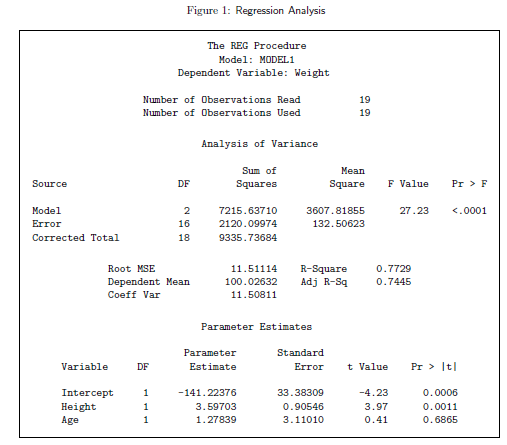
\includegraphics[width=0.8\textwidth]{images/example_output}
\end{snugshade}
\end{figure}

\definecolor{shadecolor}{rgb}{0.97,0.97,0.97}

By default, \StatRep generates listing output from the
SAS ODS Listing destination. The preceding figure provides an example
of how the SAS output is displayed in your LaTeX document.

%%%%%%%%%%%%%%%%%%%%%%%%%%%%%%%%%%%%%%%%%%%%%%%%%%%%%%%%%%%%%%%%%%%
%%%%%%%%%%%%%%%%%%%%%%%%%%%%%%%%%%%%%%%%%%%%%%%%%%%%%%%%%%%%%%%%%%%
\chapter{Syntax}

     The \StatRep package provides two environments and two tags that work
     together to display your SAS code and results and generate the SAS program
     that produces those results.

     The environments:
     \begin{itemize}
     \item The \Code{Datastep} environment contains SAS code blocks that produce no output.
     Its purpose is to read in data.
     \item The \Code{Sascode} environment contains SAS code that generates output to be
     captured. It supports line-based commands to identify
     code lines that should only be displayed, only passed to the generated program,
     or both displayed and passed to the generated program.
     \end{itemize}

     The tags:
     \begin{itemize}
     \item The \cs{Listing} tag provides information to the generated program about
     which tabular SAS output should be captured.
     It also provides information to \LaTeX\  about how that output should be displayed.
     \item The \cs{Graphic} tag provides information to the generated program about
     which graphical SAS output should be captured.
     It also provides information to \LaTeX\ about how that output should be displayed.
     \end{itemize}

     The environments and tags are described in detail in the following sections.

\section{Code Environments}

\subsection{Datastep Environment}\index{Datastep environment}

The purpose of the \Code{Datastep} environment is to read in data.
It produces no SAS results.

  The \Code{Datastep} contents are passed unchanged to the generated program.
  The \Code{Datastep} block is indented by three spaces in the PDF file.
  You can adjust the amount that the block is indented; see
  section \ref{custom} for details. The block indent is provided automatically so that
  your data and program lines can begin in the first column in your \LaTeX\ source.

  Because you begin the \Code{Datastep} data lines in the
  first column, formatted or column input statements will work correctly when
  pasted into a SAS session.\index{copy and paste}\index{interactive SAS session}


  Although the purpose of the \Code{Datastep} environment is to read in data,
  \index{reading data}%
  it can contain any SAS code that does not generate output
  to be captured.  Additional statements typically include
  TITLE and OPTIONS statements and PROC FORMAT steps. See Figure \ref{fig:sd2}
  on page \pageref{fig:sd2} for an example.


Table \ref{dsopt} summarizes the \Code{Datastep} environment options.
\index{Datastep environment!options}
\index{program option}\index{display option}\index{first= option}\index{last= option}%
\index{fontsize= option}

\begin{table}[H]
\caption{Commonly Used \Code{Datastep} Environment Options}\label{dsopt}
\begin{tabular}{lP{3.75in}}
\hline
\textbf{Option}  &  \textbf{Action} \\
\hline
                    & By default, all lines are displayed and written to the program.
\\[0.5\baselineskip]
\Code{program}      &
                 Specifies that all lines in the environment
                 be written to the generated program only
                (that is, no lines are displayed). This option is useful when you need
                to produce a data set that is not central to the topic being
                discussed and does not need to be displayed.
\\[0.5\baselineskip]
\Code{display}      &
                Specifies that all lines in the environment be displayed
                only (that is, no lines are written to the program). This option is
                useful when you need to show code fragments that will not run as is or
                example code that is not needed
                for later output generation. A \Code{Datastep} environment that specifies
                the \Code{display} option is similar to a plain \Code{verbatim} environment except
                that it is automatically indented when displayed.
\\[0.5\baselineskip]
\Code{first=\textit{n}} &
               Specifies that the first \textit{n} lines
               in the environment be displayed. The option affects only the displayed
               code block.
               This option is useful when you have many data lines that do not need to be
               displayed, but that must be available to the program.
               After the \textit{n}th line is displayed, the following
               text line is written in the displayed code block:
               \par\texttt{... more data lines ...}\par%
               You can specify different text to be used;
               see section \ref{custom} for details.
\\[0.5\baselineskip]
\Code{last=\textit{m}} &
               Specifies that the last \textit{m} lines
               in the environment be displayed. The option affects only the displayed
               code block.
               This option is used in conjunction with the \Code{first=} option to show
               the ending lines of the \Code{Datastep} environment. Without the \Code{first=}
               option, the \Code{last=} option has no effect.
\\[0.5\baselineskip]
\Code{fontsize=}   & Specifies the \LaTeX\ font size used to display the
       code block. For exampe, \Code{fontsize=small} or \Code{fontsize=footnotesize}.
\\
\hline

\end{tabular}
\end{table}

See the section \titleref{dsex} for an example.

  \subsection{Sascode Environment}\index{Sascode environment}

The purpose of the \Code{Sascode} environment is to generate output.
In addition to the environment options, it supports
line commands that enable you to specify certain lines as display-only or program-only.

 The \Code{Sascode} environment is parsed for line commands, and the appropriate lines are
 passed to the program and displayed. The displayed code block is indented by three spaces.
  You can adjust the amount the block should be indented; see section \ref{custom} for
  details.\index{display option} The block indent is provided
  automatically so that your program lines can begin in the first column in your \LaTeX\ source.

  Because all line commands are valid SAS statements,
  you can copy \Code{Sascode} blocks and paste them directly
  into a SAS session.\index{copy and paste}\index{interactive SAS session}

Table \ref{scopt} summarizes the \Code{Sascode} environment options.
\index{Sascode environment!options}\index{store= option}\index{program option}%
\index{display option}\index{fontsize= option}%

\begin{table}[H]
\caption{Commonly Used \Code{Sascode} Environment Options}\label{scopt}
\begin{tabular}{lP{3.75in}}
\hline
\textbf{Option}  &  \textbf{Action} \\
\hline
& By default, all lines are displayed and written to the program. \\[0.5\baselineskip]
\Code{store=}      &
         Specifies the name of the ODS document to contain the SAS output.
\\[0.5\baselineskip]

\Code{program}     & Specifies that  all lines in the environment
                     be written to the program only
                (that is, no lines are displayed). This option is useful when you need
                to execute code that is not central to the topic being discussed and need not
                be displayed.
\\[0.5\baselineskip]
\Code{display}     &
                  Specifies that all lines in the environment
                  be displayed only (that is, no lines are written to the program).
                This option is
                useful when you need to show example code
                fragments that will not run as is or that are not needed
                for later output generation. A \Code{Sascode} environment that specifies
                the \Code{display} option is similar to a plain \Code{verbatim} environment except
                that it is automatically indented when displayed.
\\[0.5\baselineskip]
\Code{fontsize=}   &
        specifies the \LaTeX\ font size used to display the
       code block (for example, \Code{fontsize=small} or \Code{fontsize=footnotesize}).
\\
\hline
\end{tabular}
\end{table}

The \Code{Sascode} environment also supports
a finer degree of control with line-based commands to identify lines that should
be only displayed or only passed to the generated program.

Table \ref{lcmd} summarizes the line commands you can use in the \Code{Sascode} environment.
\index{Sascode environment!line commands}
\index{program line command}\index{display line command}

\begin{table}[H]
\caption{\Code{Sascode} Line Commands}\label{lcmd}
\begin{tabular}{lP{3.5in}}
\hline
\textbf{Option}  &  \textbf{Action} \\
\hline
 \Code{\%* program} \textit{n} \Code{;} & The next \textit{n} lines are only written to
                                          the program and not displayed.\\[0.5\baselineskip]
 \Code{\%* display} \textit{n} \Code{;} & The next \textit{n} lines are only displayed
                                          and not written to the program.\\[0.5\baselineskip]
 \Code{\%*;} \textit{code line}  & The current line is only written to the
                                      program and not displayed.\\
\hline
\end{tabular}
\end{table}

  The \Code{Sascode} environment is parsed for line commands before being written
  to the generated program file.

See the sections \titleref{scex} and \titleref{scexlc} for examples.


  By using a combination of environment options and line commands, you have
  complete control over the displayed code and the generated program contents.

\section{Outputs}
     \index{SAS ODS outputs}\index{Listing tag}\index{Graphic tag}
The \cs{Listing} and \cs{Graphic} tags specify the outputs to be displayed.
The purpose of the \cs{Listing} tag is to display tabular output and notes.
The purpose of the \cs{Graphic} tag is to display graphical output.

     All figures are centered. If the figure width is narrower than the text block, the
     figure is centered with respect to the text block. Otherwise, the figure is
     centered with respect to the page.

     The \cs{Listing} and \cs{Graphic} tags support a set of options and have one
     mandatory argument, which specifies the filename prefix for the output
     to be generated and displayed.
     The prefix must be unique; otherwise the output from one example will
     overwrite another.

     Furthermore, the prefix must not end in a numeral so that the prefix name does not interfere
     with SAS-generated output file names.
    When SAS generates a set of files from one ODS selection, it follows a
    pattern: the first file that is generated is identical to the filename, the next
    file that is generated has the same name with a ``1'' appended to it, the next file
    has the same name with a ``2'' appended, and so on.

     The options supported by the \cs{Listing} and \cs{Graphic} tags are used by
     the \StatRep \LaTeX\ package and by the \StatRep SAS macros.

     The following table lists all options. Subsequent tables provide descriptions
     for each option and how it is used in LaTeX and in SAS.
\begin{table}[H]
\caption{Master List of Output Tag Options}
     \begin{tabular}{lll}
     \toprule
     \textbf{Option Name} & \textbf{Used by} & \textbf{Output Tag}\\
     \midrule
\Code{caption=}    &  LaTeX        & Listing, Graphic \\
\Code{dest=}       &  LaTeX, SAS   & Listing \\
\Code{dpi=}        &  SAS          & Graphic \\
\Code{firstobj=}   &  SAS          & Listing, Graphic \\
\Code{fontsize=}   &  LaTeX        & Listing (ODS Listing destination) \\
\Code{height=}     &  SAS          & Graphic \\
\Code{lastobj=}    &  SAS          & Listing, Graphic \\
\Code{linesize=}   &  LaTeX, SAS   & Listing (ODS Listing destination) \\
\Code{objects=}    &  SAS          & Listing, Graphic \\
\Code{options=}    &  SAS          & Listing, Graphic \\
\Code{pagesize=}   &  SAS          & Listing \\
\Code{pattern=}    &  SAS          & Listing, Graphic \\
\Code{scale=}      &  LaTeX        & Graphic \\
\Code{store=}      &  LaTeX, SAS   & Listing, Graphic \\
\Code{style=}      &  SAS          & Listing (ODS LaTeX destination), Graphic \\
\Code{type=}       &  SAS          & Listing, Graphic \\
\Code{width=}      &  LaTeX, SAS   & Graphic \\
\bottomrule
\end{tabular}
\end{table}

     \subsection{Options Used by the \textsf{StatRep} \LaTeX\ Package}
     \index{Listing tag!options}\index{Graphic tag!options}
  The following options are used by the \StatRep \LaTeX\ package.
  \index{caption= option}\index{fontsize= option}\index{linesize= option}%
  \index{scale= option}\index{store= option}\index{width= option}

  \begin{description}
     \item[\Code{caption=}] specifies the caption to use for an output.

     \item[\Code{dest=}] specifies the ODS destination to use for generating the output.
     The default value is \Code{listing}. The other possible value is \Code{latex}, which
     specifies that Listing output be generated and displayed as LaTeX tables.

     \item[\Code{fontsize=}] specifies the \LaTeX\ font size to use to display an output
    (for example, \Code{fontsize=small} or \Code{fontsize=footnotesize}).

     \item[\Code{linesize=}] specifies the line size used to generate and display
     \Code{Listing} output. By default, the value is 80 columns.
     This specification lasts for the duration of this step. The current line size is
     restored at the end.
     Typical values are \Code{80}, \Code{96}, or \Code{120}.

     For extremely wide output tables, you can use the \Code{linesize} and \Code{fontsize}
     options together (for example, \Code{linesize=120} and \Code{fontsize=scriptsize}).
     The \Code{linesize} option affects how SAS captures the table. The \Code{fontsize}
     option specifies how \LaTeX\ displays the table.\index{linesize= option}%
     \index{fontsize= option}\index{wide output}

     \item[\Code{scale=}] specifies a factor by which to scale a \Code{Graphic} image.
     For example, specify \Code{scale=0.5} to scale the image to half its original size,
     or specify \Code{scale=2} to scale it to double its original size.

    \item[\Code{store=}] specifies the name of the ODS document that is created in a
     \Code{Sascode} environment. When you specify the \Code{store=} option,
     the \StatRep package adds the appropriate SAS macro calls to the
     generated program.

     \item[width=] specifies the width to generate and display \Code{Graphic} output
           The default is 6.4 inches, which is the standard width for ODS graphs.

  \end{description}

  \subsection{Options Passed to the  \textsf{StatRep} SAS Macros}\label{sasopts}
  \index{SAS macro options}
The \Code{store=}, \Code{linesize=}, and \Code{width=} options described in the previous
section are passed to the \StatRep SAS macros.
\index{dpi= option}\index{firstobj= option}\index{height= option}\index{lastobj= option}
\index{linesize= option}\index{objects= option}\index{options= option}
In addition, the following options are passed to the \StatRep SAS macros:
  \begin{description}

  \item[\Code{dest=}] specifies the ODS destination to use for generating the output.
     The default value is \Code{listing}. The other possible value is \Code{latex}, which
     specifies that Listing output be generated and displayed as LaTeX tables.

    \item[\Code{dpi=}] specifies dots per inch (DPI) to use in generating graphs.
  The default is \Code{dpi=300}. A typical alternative is \Code{dpi=100}.

  \item[\Code{firstobj=}] specifies the first data object to capture in an output stream.
  All objects after and including the specified object
  are displayed, up to the final object
 (or optionally up to the object specified in \Code{lastobj=}).
  You can use \Code{options=skipfirst} to begin with the object after the one specified in \Code{firstobj=}.
  See section \ref{selection} for details.

  \item[\Code{height=}] specifies the height of graphs. The default is 0.75 times the width.

  \item[\Code{lastobj=}] specifies the last data object to capture in an output stream.
  All objects starting with the first object
  (or optionally the object specified in \Code{firstobj=}) are displayed up to and
  including the specified object.
  You can use \Code{options=skiplast} to end with the object before the one specified in \Code{lastobj=}.

\item[\Code{linesize=}] specifies the line size used to generate and display
     \Code{Listing} output. By default, the value is 80 columns.
     This specification lasts for the duration of this step. The current line size is
     restored at the end.
     Typical values are \Code{80}, \Code{96}, or \Code{120}.

  \item[\Code{objects=}] specifies a space-separated list of ODS objects to capture
  in an output stream.
  The names that are used for selection come from the ODS document.
  If you specify \Code{objects=}, then you can also specify object breaking rules
  (where page breaks can occur). See section \ref{selection} for details.

  \item[\Code{options=}] specifies binary options.  Specify one value or a space-separated
  list of values (for example, \Code{options=skipfirst skiplast}).
  You can specify the following values (the default is \Code{options=autopage}):

  \begin{description}
  \item[\Code{autopage}] specifies that the first \cs{Listing}
  command or \Code{\%write} macro start a new output stream with
  titles, procedure titles, and so on.
  Page breaks also occur at other places where the procedure
  explicitly sets a page break. The \Code{autopage} value is the default.
  See also the \Code{nopage} and \Code{newpage} values.
  \index{autopage option}

 \item[\Code{graph}] specifies that only graphs be selected.
  You can alternatively specify \Code{type=graph}.\index{graph option}

  \item[\Code{list}] specifies that the contents of the ODS document be listed
  in the SAS log. This value does not run PROC DOCUMENT to replay the output.\index{list option}

  \item[\Code{newpage}] specifies that SAS force a new page for the first object.
  \index{newpage option}

  \item[\Code{nopage}] suppresses page breaks.\index{nopage option}

  \item[\Code{onebox}] groups all tables, notes, reports, and so on into a
  single piece of SAS output. You cannot specify this option to group graphs.
  See section \ref{selection} for more information about grouping.\index{onebox option}

  \item[\Code{skipfirst}] modifies the \Code{firstobj=} option so that the first object in the
  list is not selected. This enables you to select all objects after the one
  specified in \Code{firstobj=}.\index{skipfirst option}

  \item[\Code{skiplast}] modifies the \Code{lastobj=} option so that the last object
  in the list is not selected. This enables you to select all objects before
  the one specified in \Code{lastobj=}.\label{skiplast}\index{skiplast option}

  \item[\Code{table}] selects all objects
  (tables, notes, reports, and so on) except graphs. You can
  alternatively specify \Code{type=listing}.\index{table option}

  \end{description}

  \item[\Code{pagesize=}] specifies the page size. The default is the page size currently in effect.
  This specification lasts for the
  duration of this step. The current page size is restored at the end.\index{pagesize= option}

  If you have not changed the page size, the default page size set by the \StatRep
  package is 500. This large page size is the default so that output is generated with
  minimal new pages caused by page boundaries. For large tables, you can specify a smaller
  page size to force more page breaks. See section \ref{custom} for information about
  how to change the \StatRep default. See section \ref{large} for information about how
  to use the \Code{pagesize=} option with large tables.

  \item[\Code{pattern=}] provides an optional and additional selection criterion.
  Specify part of a path (for example, a group name).\index{pattern= option}
  Only objects whose name includes the specified value are selected.

    \item[\Code{store=}] specifies the name of the ODS document that is created in a
     \Code{Sascode} environment. When you specify the \Code{store=} option,
     the \StatRep package adds the appropriate SAS macro calls to the
     generated program.\index{store= option}

  \item[\Code{style=}] specifies the ODS style to use in generating output.
    The default is \mbox{\Code{style=Statistical}}. You can change the default style
    (for example, to \Code{HTMLBlue}) by inserting the following line into a \Code{Sascode}
    or \Code{Datastep} environment:\index{style= option}

\begin{snugshade}
\begin{verbatim}
 *; %let defaultstyle=HTMLBlue;
\end{verbatim}
\end{snugshade}

    This option affects ODS graphs only when used in a \cs{Graphic} tag.
    You can specify this option in the \Code{\%output} macro to set the style
    for GRSEG graphs (graphs that are produced by legacy SAS/GRAPH
    procedures such as the GPLOT, GMAP, and GCHART procedures).
    GRSEG graphs are stored in catalogs
    and cannot be changed after they are generated. In contrast,
    style, DPI, and so on for ODS graphis can be changed after the graph is initially created.
    See section \ref{grseg} for more information.

 \item[\Code{type=\emph{listing}|\emph{graph}}] specifies that only listings or
  only graphs be selected.
  You can alternatively specify \Code{options=table} or \Code{options=graph}.
      \item[\Code{width=}] specifies the width to generate and display \Code{Graphic} output
           The default is 6.4 inches, which is the standard width for ODS graphs.

  \end{description}



%%%%%%%%%%%%%%%%%%%%%%%%%%%%%%%%%%%%%%%%%%%%%%%%%%%%%%%%%%%%%%%%%%%
%%%%%%%%%%%%%%%%%%%%%%%%%%%%%%%%%%%%%%%%%%%%%%%%%%%%%%%%%%%%%%%%%%%
\chapter{Details}

The preceding pages should provide the information to use the package
in most scenarios. For more in-depth descriptions and methods for
customization, see the following sections.

\begin{description}
\item[Customizing \StatRep] describes several hooks for customizing
the package and setting system-wide defaults.
\item[The Program Preamble] provides an overview of how the \StatRep
package works with the SAS macros; a special file (the program preamble)
provides a method of communication between the two.
\item[Two Methods of Writing] describe how you can bypass the automatic
code generation and use the \StatRep SAS macros directly.
\item[\StatRep SAS Macros] describe in detail each SAS macro in the
\StatRep package. You can use these macros yourself for maximum flexibility
in creating a custom \StatRep document.
\item[ODS Object Selection] describes how you can use options in the
\cs{Listing} and \cs{Graphic} tag to specify exactly what output you want
to display.
\item[ODS Graphics] describes differences between ODS graphics and
GRSEG graphics.
\end{description}

 \section{Customizing \StatRep}\label{custom}
 \index{customizing}\index{configuration}

  You can modify the configuration file \Code{statrep.cfg} to change
the following settings used by the \StatRep package.
  See section \ref{secdefaults} for more information about macro variable defaults.

    \begin{description}
     \item[\cs{SRcaptionfont}] specifies the font for the output captions.
     The default is \cs{sffamily} (\textsf{sans serif}).
     \index{caption font}

     \item[\cs{SRcaptioncontinuedfont}] specifies the font for the \Code{continued} name
     for outputs that break across pages.
     The default is \cs{sffamily}\cs{itshape} (\textsf{\textit{sans serif, italic}}).

     \item[\cs{SRcontinuedname}] specifies the name that indicates that an output
     block is continued. The name is used when an output stream breaks across a page.
     The default is \Code{continued}.

    \item[\cs{SRdefaultdests}] specifies the default ODS Destination for tabular
    outputs. The default is \Code{listing}. You can specify \Code{latex} to produce
    SAS-generated LaTeX tabular output. See section \ref{latexoutput} for details.
    \index{LaTeX output}

    \item[\cs{SRdpi}] specifies the default dots per inch (DPI) for SAS to use in generating
    graphical output. The default is \Code{300}.
    \index{dpi}

    \item[\cs{SRgraphicdir}] specifies the name of the directory that contains the SAS
     generated graphical output files. The default is \Code{png}.
     \index{graphic directory}

    \item[\cs{SRgraphtype}] specifies the format of the SAS
     generated graphical output. You can specify either
     \Code{png} or \Code{pdf}. The default is \Code{png}.
     \index{graphics type}\index{PNG graphics}\index{PDF graphics}

    \item[\cs{SRlatexdir}] specifies the name of the directory that contains the
    SAS generated LaTeX tabular output. The default is \Code{tex}.
    See section \ref{latexoutput} for details.

    \item[\cs{SRlatexstyle}] specifies the ODS style for SAS to use to generate
    LaTeX tabular output. The default is \Code{statrep}, a monochromatic style based
    on the \Code{statistical} ODS style.
    See section \ref{latexoutput} for details.

    \item[\cs{SRodsgraphopts}] specifies a string that is passed as
    ODS GRAPHICS statement options. For a complete explanation of all available options,
    see the documentation of the ODS GRAPHICS statement in
    \textit{SAS Output Delivery System: User's Guide}.
    \index{ODS graphics options}

    \item[\cs{SRintertext}] specifies the text to insert in
    \Code{Datastep} environments that specify
     the \Code{first=} option. The default is \Code{\mbox{... more data lines ...}}

    \item[\cs{SRlinesize}] specifies the default line size to use in generating tabular
    output and centering it for display. The default is \Code{80}.
    \index{output width}\index{linesize}

     \item[\cs{SRlistingdir}] specifies the name of the directory that contains the SAS
     generated listing (tabular) output files. The default is \Code{lst}.

     \item[\cs{SRmacropath}] specifies the path to the location of the
     SAS macros that are bundled with the \Code{StatRep} package.
     \index{SAS macro location}
     For example, if  you installed the \Code{statrep\_macros.sas} file to a directory named
    \Code{C:\textbackslash mymacros},
    then define macro \cs{SRmacropath} as follows:
    \begin{verbatim}
    \def\SRmacropath{c:/mymacros/statrep_macros.sas}
    \end{verbatim}

   Use the forward slash in the definition
   as the directory name delimiter instead of the backslash, which is a special
   character in \LaTeX. If you want to use a backslash character (\textbackslash), you
   must insert it with the \LaTeX\ command, \cs{@backslashchar}.

   The default value is the current path. That is, the default
   definition for the \cs{SRmacropath} macro is the filename itself, \Code{statrep\_macros.sas}.

     \item[\cs{SRmacroinclude}] specifies the line used in the generated SAS program to
     include the SAS macros that are bundled with the \Code{StatRep} package.
     The default is\\\Code{\%include }\cs{SRmacropath}~\Code{/nosource;}

    \item[\cs{SRpagesize}] specifies the default page size for SAS to use in generating
    tabular output. The default is \Code{500}.


     \item[\cs{SRparindent}] specifies the amount of space to indent
     \Code{Datastep} and \Code{Sascode} environments.
     The argument is a dimension.
     The default is \Code{3em} and is measured according to the font currently in use.

     \item[\cs{SRprogramline}] specifies the first lines to include in the generated SAS program
     after the \cs{SRmacroinclude} line.

     The following default value calls a macro (from \Code{statrep\_macros.sas})
     that removes the contents of the listing and graphic directories to ensure
     that the generated graphs and listings from the SAS program are current.
     The directories are created with
     each SAS run that includes the macros themselves (via \Code{x} commands).
\begin{snugshade}
\begin{verbatim}
   %hostdel;
\end{verbatim}
\end{snugshade}

      \item[\cs{SRprogramname}] specifies the filename for the generated SAS
     program. The default is \cs{jobname\_SR.sas}, where \cs{jobname} is
     usually the stem name of the \LaTeX\ source file.


    \item[\cs{SRstyle}] specifies the default ODS style for SAS to use to generate
    graphical output. The default is \Code{Statistical}.
    \index{ODS output style}

     \item[\cs{SRtempfilename}] specifies the name of a temporary file
     that is used as a scratch file in the current working directory.
     The default is \Code{sr.tmp}.

     \item[\cs{SRverbfont}] specifies the font to use for code within \Code{Datastep} and
     \Code{Sascode} blocks. The default is \cs{ttfamily}\cs{bfseries}
     (\texttt{\textbf{typewriter text, bold}}).
     \index{verbatim font}

     \end{description}

  \section{The Program Preamble}

The \StatRep package automatically writes a preamble to the generated program and a preamble file.

The preamble settings are split into two parts to support users who prefer to
manually write the calls to the \StatRep macros and work interactively between the
\LaTeX\ source document and a SAS session.  For this use, you can include the external
preamble file once in your SAS session and all the necessary settings are made for you.

If you do not manually write calls to the \StatRep macros (you use the default, automated method),
there is nothing you need to do---your generated program contains the lines that specify your settings.

The preamble in the generated program includes the preamble file and deletes the contents of the
output directories (\Code{lst}, \Code{tex}, and \Code{png}, by default) so that obsolete files are
not included in the document.
Figure \ref{fig:pgmpreamble} shows an example of the preamble lines
that are written to the generated program.
\begin{figure}[H]
\begin{snugshade}
\begin{verbatim}
/*
 This file is auto-generated by the statrep package.
 Do not edit this file or your changes will be lost.
 Edit the LaTeX file instead.

 See the statrep package documentation and the file
 statrep.cfg for information on these settings.
 */


%include "report_SR_preamble.sas" /nosource;
/* Remove all output files. */
%hostdel;

/* Start program with a null title. */
title;
\end{verbatim}
\end{snugshade}
\caption{Generated SAS Program Preamble}\label{fig:pgmpreamble}
\end{figure}

  The external preamble file sets defaults, includes
  the output-capture macros, and creates the output directories if they do not exist.
  You can customize the preamble; see section \ref{custom} for details.
  Figure \ref{fig:preamble} shows the default file preamble.
\begin{figure}[H]
\begin{snugshade}
\begin{verbatim}
/*
 This file is auto-generated by the statrep package.
 Do not edit this file or your changes will be lost.
 Edit the LaTeX file instead.

 See the statrep package documentation and the file
 statrep.cfg for information on these settings.
 */


/* Set and invoke macro variable defaults. */
%let defaultlinesize=80;
%let defaultpagesize=500;
%let defaultdpi=300;
%let defaultstyle=statistical;
%let listingdir=lst;
%let graphicdir=png;
%let graphtype=png;
%let odsgraphopts=;
%let latexdir=tex;
%let latexstyle=statrep;
%let defaultdests=listing;

options nodate nonumber
ls=&defaultlinesize ps=&defaultpagesize
formchar='|----|+|---+=|-/\<>*';

ods graphics on;
/* Include SAS macro definitions. */
%include "statrep_macros.sas" /nosource;

\end{verbatim}
\end{snugshade}
\caption{Generated Preamble File}\label{fig:preamble}
\end{figure}

\section{Two Methods of Writing}
  To maximize flexibility, the \StatRep package provides two methods of writing code in your
\LaTeX\ document.

When you create your \LaTeX\ document, you can use either the automatic method described in
section \ref{gs} (in which the SAS macro calls are generated automatically) or a manual
method (in which you write the \Code{\%output}, \Code{\%endoutput}, and \Code{\%write} macros yourself).

In the automatic method, each \Code{Sascode} code block generates an \Code{\%output} macro call at the beginning
of the block and an \Code{\%endoutput} macro call at the end of the block.
Each \cs{Listing} and \cs{Graphic} tag generates the \Code{\%write}
macro to replay the selected output objects to external files.

In the manual method, you decide where and when to make the macro calls.
It is only in this respect that the method is manual: the
\StatRep package still generates your SAS program and displays your code and results.

The \StatRep package uses
  the SAS macro comment (\Code{\%* \emph{comment} ;}) to provide line
  commands within a \Code{Sascode}
  block. Furthermore, any line of code that begins with a null macro
  comment (\Code{\%*;})
  is written to the SAS program and is not displayed.

You can use the manual method when you want to do one or more of the following:
\begin{itemize}
\item capture specialized or complicated output
\item capture print output with SAS 9.2 (see the \Code{\%startlist} macro in section \ref{startlist})
\item capture output from the SAS log (see the \Code{\%startlog} macro in section \ref{startlog})
\item work interactively when writing (you can interactively develop or debug a
        certain section of your document by copying code from
        your \LaTeX\ document and pasting it into a SAS session)
\end{itemize}

 You can use either method, and you can
mix the methods in a single document. The manual method is provided for cases in which the
automatic method is too inflexible. By using the line commands in a \Code{Sascode} environment,
you are free to write your program as you want, while retaining control of the code that is
displayed in your final PDF document.

  Continuing with example shown in Figure \ref{fig:d1} and Figure \ref{fig:s1},
  you can write the code yourself within your
  \LaTeX\ document as shown in Figure \ref{fig:manual}
  and obtain the identical code display and capture.

\begin{figure}[H]
\begin{framed}
\begin{snugshade}
{\hfil\textit{Datastep is identical}\hfil}
\begin{verbatim}
\begin{Datastep}
proc format;
   value $sex 'F' = 'Female' 'M' = 'Male';
data one;
   set sashelp.class;
   format sex $sex.;
run;
\end{Datastep}
\end{verbatim}
\end{snugshade}
\begin{snugshade}
{\hfil\textit{\texttt{\%output} added manually}\hfil}
\begin{verbatim}
\begin{Sascode}
 *; %output(class)
proc reg;
    model weight = height age;
run;
\end{verbatim}
\end{snugshade}
\begin{snugshade}
{\hfil\textit{\texttt{\%write} macros added manually}\hfil}
\begin{verbatim}
 *; %write(rega, type=listing)
 *; %write(regb, type=graphic)
\end{Sascode}
\end{verbatim}
\end{snugshade}
\begin{snugshade}
{\hfil\textit{Listing and Graphic tags only caption and insert output}\hfil}
\begin{verbatim}
\Listing[caption={Regression Analysis}]{rega}
\Graphic[caption={Graphs for Regression Analysis}]{regb}
\end{verbatim}
\end{snugshade}
\end{framed}
\caption{Using the SAS Macros Manually}\label{fig:manual}
\end{figure}

  The \Code{Datastep} environment in Figure \ref{fig:manual} is identical to that shown in the
  Figure \ref{fig:d1}. However, the \Code{Sascode}
  environment makes an explicit call to the \Code{\%output} macro to create
  the ODS document that contains all the results from the code block.
  Because this line begins with the null SAS macro comment (\Code{\%*;}), the line
  is passed directly to the generated SAS program and is not displayed.

  The \Code{\%endoutput} macro is not necessary when you are processing
  only one ODS document. It is implicitly specified by the first \Code{\%write} macro.

  Next are two explicit calls to the \Code{\%write} macro, which
  specify the ODS objects to capture and the ODS document that the objects
  should be taken from.
  Both \Code{\%write} macros use the minimum number of options.
  The first \Code{\%write} macro selects all
  notes and tables from the last ODS document created. The second \Code{\%write} macro
  selects all graphs from the last ODS document created.
  Because the \Code{store=} option is omitted in both cases,
  output from the most recently created ODS document is displayed.

  Finally, the \cs{Listing} and \cs{Graphic} tags request the outputs.
  In
  this method, you do not place the options that are related to SAS in the
  the \cs{Listing} and \cs{Graphic} tags. You need to
  specify only the caption and filename prefix.


  To summarize, the \Code{Datastep} environment is handled identically in either method,
  the \Code{Sascode} environment can optionally produce the \Code{\%output} and \Code{\%endoutput} macros,
  and the \cs{Listing} and \cs{Graphic} tags can optionally produce the \Code{\%write} macros.

\section{\StatRep SAS Macros}\label{macros}
\index{SAS macros}
  SAS programs created by the \StatRep package
  run SAS macros to capture output. The macros depend on the ODS document.
  The ODS document is a destination or repository for the results
  (tables, notes, titles, and graphs)
  that come from SAS procedures. Each procedure step is run only once,
  and the results are captured in an ODS document.
  Then the parts of the ODS document are replayed using PROC DOCUMENT.

  When \StatRep encounters a \Code{Sascode} environment,
  it generates a macro call to create an ODS document from the environment.
  When \StatRep encounters a \cs{Listing} or \cs{Graphic} tag,
  it generates a macro call to replay output from that ODS document into an external file.

  For the output that is generated in each \Code{Sascode} block, the SAS macros provide you
  with a list of all
  of the objects in the ODS document and a table that displays
  the objects selected for display. You can
  review this list in the SAS log.
  It is important to check these lists to ensure that either all output
  is included somewhere or any omissions are deliberate.

  The following macros are defined:
  \begin{itemize}
  \item The \Code{\%output} and \Code{\%endoutput} macros open and close an ODS document, respectively.
  When you use \StatRep to automatically generate your program, these macros are called at the
  beginning and end of a \Code{Sascode} block, respectively.
  You can manually call the macros at any time within
  a \Code{Sascode} block by prefixing the call with a null SAS macro comment (\Code{\%*;}).
  \index{SAS macros!output}\index{SAS macros!endoutput}

  \item The \Code{\%write}  macro writes ODS objects that are contained in an ODS document to
  one or more external files.
  When you use \StatRep to automatically generate your program, this macro is called when
  a \cs{Listing} or \cs{Graphic} tag is encountered. You can manually call the macro
  at any time within a \Code{Sascode} block by prefixing the call with a null
  SAS macro comment (\Code{\%*;}).
  \index{SAS macros!write}

  \item The \Code{\%startlist} and \Code{\%endlist} macros capture printed content
  (for example, a PROC PRINT or DATA step) to an external file. To use these macros,
  you must manually call the macro
  within a \Code{Sascode} block and prefix the call with a null
  SAS macro comment (\Code{\%*;}).
  \index{SAS macros!startlist}\index{SAS macros!endlist}

  \item The \Code{\%startlog} and \Code{\%endlog} macros capture content from the
  SAS log to an external file. To use these macros,
  you must manually call the macro
  within a \Code{Sascode} block and prefix the call with a null
  SAS macro comment (\Code{\%*;}).
  \index{SAS macros!startlog}\index{SAS macros!endlog}
  \end{itemize}


  \subsection{The \texttt{\%output} and \texttt{\%endoutput} Macros}\label{outputmacro}
  The \Code{Sascode} environment writes the \Code{\%output} and \Code{\%endoutput} macros to
  the generated program
  whenever the \Code{store=} option is specified.
  However, you can call the macros
  yourself by omitting the \Code{store=} option in the \Code{Sascode} environment and
  call the macros within the \Code{Sascode} environment. Each call must be prefixed
  with a null SAS macro comment (\Code{\%*;}).
  \index{SAS macros!output}\index{SAS macros!endoutput}

  The \Code{\%output} macro supports two other options (\Code{style=} and \Code{dpi=}) that are used to
  set parameters for GRSEG graphs. These options are not supported in the
  \Code{Sascode} environment options. If you want to change the style or DPI for
  GRSEG graphs, you must call the \Code{\%output} and \Code{\%endoutput} macros manually.

  The following options are supported by the \Code{\%output} macro:
 \begin{description}
 \item[\Code{store=}] specifies the name of the ODS document.
  This name is used in the \Code{store=} option in the \cs{Listing} and \cs{Graphic} tags
  or in the \Code{\%write macro}.

 \item[\Code{style=}] specifies the style used for GRSEG graphs.
 The default is \Code{HTMLBlue}. See section \ref{grseg} for details.

 \item[\Code{dpi=}] specifies the dots per inch (DPI) setting used for GRSEG graphs.
  The default is 300 DPI. See section \ref{grseg} for details.
 \end{description}


  \subsection{The \texttt{\%write} Macro}
  The \Code{\%write} macro supports the same key-value options as the \cs{Listing} and
  \cs{Graphic} tags support.
  The \StatRep package generates the \Code{\%write} macro in the SAS program
  file whenever the \Code{store=} option is specified in the output tag.
  However, you can call the macros
  yourself by omitting the \Code{store=} option in the \cs{Listing} or \cs{Graphic}
  tag and call the macro within a \Code{Sascode} environment. Each call must be prefixed
  with a null SAS macro comment (\Code{\%*;}).
  \index{SAS macros!write}
See the section \titleref{sasopts} for more information about the options used in the
\cs{Listing} and \cs{Graphic} tags that are passed to the \Code{\%write} macro.


\vspace*{1em}\noindent\textbf{Note:} If you use the macros interactively, be aware that
these macros open and close ODS destinations,
enable and disable ODS Graphics, and change ODS options.  Output capture uses the
LISTING destination, and when the \Code{\%write} macro finishes, only the
LISTING destination remains open.
If you need other ODS destinations for your work, you need to reset them
when you are done with a section of output capture.  For example,
if you are using the HTML destination
in the SAS windowing environment, then you need to
close the LISTING destination and reopen the HTML destination when you finish
capturing output.

 \subsection{The \texttt{\%startlist} and \texttt{\%endlist} Macros}\label{startlist}

  The \Code{\%startlist} and \Code{\%endlist} macros capture printed information
  from the ODS listing destination. The macros are used when
  you create output with a procedure that does not support ODS.
  They are also used when you use the
  \Code{DATA \_NULL\_} and \Code{PUT \_ODS\_} SAS statements to
  manually capture output.
  \index{SAS macros!startlist}\index{SAS macros!endlist}

  These macros are not automatically generated by the \StatRep package.
  You must call them
  manually within a \Code{Sascode} environment (with each call preceded
  by a null SAS macro comment).

  In SAS 9.2, PROC PRINT is not fully integrated into the ODS document,
  unless you specify PROC PRINT with no options.
  If you specify PROC PRINT
  with options, you must use the \Code{\%startlist} and \Code{\%endlist}
  macros to capture output.

  If you use PROC PRINT in SAS 9.3 or later,
  you can use the \Code{\%output} and \Code{\%write} macros as you would with
  any SAS procedure.

  The \Code{\%startlist} macro has one mandatory argument, the filename prefix
  of the file to contain
  the output. The argument is also used
  in the \cs{Listing} tag to insert the output.

  The \Code{\%startlist} macro supports the following options after
  the filename argument, separated with a comma (,):
  \begin{description}
  \item[\Code{linesize=}] specifies the line size.
  The default is the line size currently in effect.
  This specification lasts for the duration of this step.
  The current line size is restored at the end.
  When you specify the \Code{linesize=} option in the \Code{\%startlist}
  macro, be sure to make the same specification
  in the \cs{Listing} tag you use to insert the output.

  \item[\Code{pagesize=}] specifies the size of the output page.
   The default is the page size currently in effect.
   This specification lasts for the duration of this step.
  The current page size is restored at the end.
  This option is useful for breaking up long listings into smaller parts to allow for page breaks.
  If a listing output spans more than one SAS page,
  the output is automatically split into parts and the page breaks
  can occur only between parts of output.
  For more information about capturing large outputs, see section \ref{large}.
  \end{description}

 \subsection{The \texttt{\%startlog} and \texttt{\%endlog} Macros}\label{startlog}

  The \Code{\%startlog} and \Code{\%endlog} macros capture SAS notes
  or error messages from the SAS log. They also capture output
  from some SAS/IML functions that write to the SAS log rather than using ODS.
  \index{SAS macros!startlog}\index{SAS macros!endlog}

  These macros are not automatically generated by the \StatRep package.
  To capture content from the SAS log, you must call these macros
  manually within a \Code{Sascode} environment (with each call preceded
  by a null SAS macro comment).

  The \Code{\%startlog} macro has one mandatory argument, the filename prefix
  of the file to contain the output. The argument is also used in the \cs{Listing}
  tag to insert the output.

  The \Code{\%endlog} macro supports the following options,
  separated by a comma (,):

  \begin{description}
  \item[\Code{code=}] specifies whether program code in the SAS log is included.
  By default, code is captured (\Code{code=1}). Set \Code{code=0} to exclude code.
  \item[\Code{range=}] specifies a Boolean expression to select
  certain observations. For example, you can specify \Code{range=\_n\_ <= 5 }
  to select the first five lines.  You can specify
  \Code{range=not index(line, 'ERROR')} to select all lines that do not contain the string
  `ERROR'. Selection must be based on \Code{\_n\_} or the variable \Code{line}, which
  contains a single line of the log.
  \end{description}

  \subsection{Macro Variable Defaults}\label{secdefaults}
  \index{macro variables}\index{default settings}\index{package!defaults}
  \index{SAS macros!variables}

  The SAS macro defaults are set globally in the file \Code{statrep.cfg}.
  See section \ref{custom} for details. You can also reset the
  defaults within your document by specifying new settings in a \Code{Sascode}
  environment.

  Table \ref{defaults} shows the description and default values for each
  macro variable.

  \begin{table}[H]
  \centering\caption{Default Values for Macro Variables}\label{defaults}
  \begin{tabular}{llP{2.5in}}
  \textbf{Macro Variable}    & \textbf{Default} & \textbf{Description}\\
  \hline
    \Code{defaultlinesize}  & 80      & Line size for tabular ODS output\\
    \Code{defaultpagesize}  & 500     & Page size for tabular ODS output\\
    \Code{defaultstyle}     & Statistical & ODS style for graphical output \\
    \Code{defaultdpi}       & 300      & Dots per inch (DPI) for graphical output\\
    \Code{graphtype}        & png      & graphics file format ('png' or 'pdf')\\
    \Code{odsgraphopts}     &          & string containing ODS graphics options\\
    \Code{defaultdests}     & listing  & \texttt{listing} or \texttt{latex} tabular output\\
    \Code{latexstyle}       & statrep  & ODS Style for SAS-generated LaTeX output\\
  \hline
   \end{tabular}
  \end{table}

  You can edit the \Code{statrep.cfg} file\index{customizing}\index{statrep.cfg}
  \index{configuration}%
  to globally reset the defaults, or you can specify commands to change the default anywhere
  in your document. For example, the following lines change all of the macro variable
  default settings for the duration of the program. The \Code{program} option specifies
  that the code be written only to the generated program and not displayed.


\begin{figure}[H]
\begin{snugshade}
\begin{verbatim}
   \begin{Sascode}[program]
   %let defaultlinesize=96;
   %let defaultpagesize=50;
   %let defaultstyle=statistical;
   %let defaultdpi=100;
   %let graphtype=pdf;
   %let odsgraphopts=antialiasmax=10000;
   \end{Sascode}
\end{verbatim}
\end{snugshade}
\caption{Reset SAS Macro Defaults within Document with SAS}\label{reset}
\end{figure}

  When you change the \Code{defaultlinesize} in the \Code{statrep.cfg} file, the same value
  is automatically used by SAS and by the \StatRep package.
  When you change the \Code{defaultlinesize} inside your document,
  you change the line size used by SAS in generating
  outputs; You must also set the line size in the \cs{Listing} tag to match.

  The setting of \Code{defaultpagesize=500} produces a large
  virtual page so that SAS does not break ODS objects into smaller pieces.
  When a stream of outputs is typeset, page breaks can occur only between ODS objects or
  when SAS forces a page break inside an ODS table.

  The macro options and default macro variables work as follows:
  If an option is specified in a macro, its value is used regardless of
  the specification in the default macro variables.
  If an option is not specified in a macro, the default macro variables provide
  the values.

  In summary, a direct option specification in a macro takes precedence over the default
  settings, and you can change the default settings by resetting the
  default macro variables
  in your document or by editing the \Code{statrep.cfg} file.

 \section{ODS Object Selection}\label{selection}
To select and display ODS objects, you specify options in the \cs{Listing} tag, \cs{Graphic}
  tag, or the \Code{\%write} macro.
\label{optionopt}
By default, when you omit object selection options, the \Code{\%write} macro selects all ODS objects,
the \cs{Listing} tag selects all ODS tables and notes, and the \cs{Graphic} tag selects all ODS graphs.
\index{ODS object selection}
  Table \ref{tabselect} summarizes how you select ODS objects.
  \begin{table}[H]
  \centering\caption{ODS Object Selection Options}\label{tabselect}
  \begin{tabular}{lP{3.75in}}
  \textbf{Option}  & \textbf{Action}\\
  \hline
  \Code{options=table}    & Select all tables and notes\\
  \Code{options=graph}    & Select all graphs \\
  \Code{pattern=} \textit{pattern}   &
Select all objects with a name matching a pattern.
When an ODS object name has more than two levels,
  the middle level name is a group name. You can specify the \Code{pattern=} option
  to select all ODS objects in the specified ODS group.
  More generally, you can specify any pattern to select all objects
  whose path contains the pattern.\\
  \Code{firstobj=} & Specifies the first object in the output stream to capture.
  The specified and subsequent objects are captured.\\
  \Code{lastobj=}  & Specifies the last object in the output stream to capture.
The first object in the stream to capture is the first object produced by the
\Code{Sascode} code block or the object specified in the \Code{firstobj=} option.\\
  \Code{objects=} option & Specifies a space-separated list of objects to capture.\\
  \hline
  \end{tabular}
  \end{table}

  The \Code{firstobj=} and \Code{lastobj=} options can be modified with the option
  \Code{options=skiplast} and  \Code{options=skipfirst}. For more information about
  how to use these options,
  see page \pageref{skiplast}.

  \subsection{Page Breaks}\label{pagebreak}
  By default, a page break can occur between any two objects in the output stream.
  However, you can use left and right angle brackets, \Code{<>},  to delineate a
  set of objects in which to suppress breaks.
  You use the symbols in the \Code{objects=} option list in
  a \cs{Listing} tag, a \cs{Graphic} tag, or a \Code{\%write} macro.


  For example, you can use the symbols to prevent a break between a
  ``Parameter Estimates'' table and the ``Fit Statistics'' table that follows it
  with the following option:
  \Code{objects = < ParameterEstimates FitStatistics >}

  After the \Code{<} symbol, breaking is suppressed until the \Code{>} symbol is encountered.
  After the \Code{>} symbol, a break is introduced and normal breaking continues.

  In summary:
  \begin{itemize}
  \item You can use the \Code{<>} symbols in pairs to keep ODS objects together.
  \item You can use the \Code{>} symbol (unpaired with a matching \Code{<}) to create a break between tables.
  \item You can use the \Code{<} symbol (unpaired with a matching \Code{>}) to suppress all breaks.
  \end{itemize}

  A break is always allowed before and after a graph.

  See page \pageref{skiplast} for an alternate method of controlling breaks
  with the \Code{options=nopage} and \Code{options=onebox} options.

 \section{ODS Graphics}
 \index{ODS graphics}

 In SAS 9.3 and later, ODS Graphics is enabled by default in the SAS windowing environment.
 ODS Graphics is not enabled by default in batch mode and in the SAS windowing environment in SAS 9.2.
 When ODS Graphics is not enabled by default, you can enable ODS Graphics by specifying the following statement:

\begin{snugshade}
\begin{verbatim}
   ods graphics on;
\end{verbatim}
\end{snugshade}


You can enable ODS Graphics in \StatRep for all steps by providing this code block at the
beginning of your LaTeX document:

\begin{snugshade}
\begin{verbatim}
   \begin{Sascode}[program]
      ods graphics on;
   \end{Sascode}
\end{verbatim}
\end{snugshade}

 \subsection{ODS Graphics and GRSEG Graphics}
 \label{grseg}
  \index{ODS graphics}\index{GRSEG graphics}
  When you create a graph with ODS Graphics, the style and dots per inch (DPI) can be changed
  after the graph is created. The style and DPI are set when the
  graph is written to the external file. This enables you to specify the options
  in the \cs{Graphic} tag or in the \Code{\%write} macro.

  On the other hand, when you create a GRSEG graph, the style and DPI
  are set when the graph is created. That is why you must specify the options
  in the \Code{\%output} macro. See section \ref{outputmacro} for details
  about the \Code{\%output} macro options.

  Table \ref{tabgraph} summarizes the methods you can use to modify the
  style and DPI settings when you create a graph.

  \begin{table}[H]
  \centering
  \caption{Methods to Change Graph Properties}\label{tabgraph}
  \begin{tabular}{lcc}
  \textbf{Method}          & \textbf{ODS Graph} & \textbf{GRSEG Graph} \\
  \hline
  \cs{Graphic} tag options &  Yes         & No    \\
  \Code{\%write} macro options   &  Yes         & No    \\
  \Code{\%output} macro options  &   No         & Yes   \\
  Reset global default     &  Yes         & Yes   \\
  \hline
  \end{tabular}
  \end{table}

  The \cs{Graphic} tag, the \Code{\%write} macro, and the
  \Code{\%output} macro have \Code{style=} and \Code{dpi=} options. For more information
  about these options, see section \ref{sasopts}.
  Also, see section \ref{secdefaults} for details about
  using the SAS macro variables to reset global defaults.

  For GRSEG graphs, there are only two choices for DPI: 300 (the default) and 96.
  When the DPI is set to anything other than 300,
  then 96 is automatically used instead for GRSEG graphs.

%%%%%%%%%%%%%%%%%%%%%%%%%%%%%%%%%%%%%%%%%%%%%%%%%%%%%%%%%%%%%%%%%%%
%%%%%%%%%%%%%%%%%%%%%%%%%%%%%%%%%%%%%%%%%%%%%%%%%%%%%%%%%%%%%%%%%%%
\chapter{Examples}

\section{Using the Datastep Environment}\label{dsex}
\index{Datastep environment}
  Figure \ref{fig:sd2} displays an example \Code{Datastep} environment. The left margin for
  the environment is in the first column, which is where the data lines themselves begin.
  This ensures that the variables will be read correctly.

\begin{figure}[H]
\begin{snugshade}
\begin{verbatim}
\begin{Datastep}[first=9, last=3]
title 'Probit Analysis, Newspaper Survey';
proc format;
   value subscrib 1 = 'accept' 0 = 'reject';
run;
data news;
   input sex $ 1-6 age 12-13 subs 18 ;
   datalines;
Female     35    0
Male       45    1
Female     51    0
Male       54    1
Female     35    0
Female     48    0
Male       46    1
Female     46    1
Male       38    1
Male       49    1
Male       50    1
Female     47    0
Female     39    0
Female     45    0
Male       39    1
Female     39    0
Female     52    1
Male       58    1
Female     32    0
Female     35    0
;
\end{Datastep}
\end{verbatim}
\end{snugshade}
\caption{\texttt{Datastep} Environment with Options}\label{fig:sd2}
\end{figure}

  In Figure \ref{fig:sd2}, the options to the \Code{Datastep} environment specify that only a portion
  of the code block be displayed.  All lines in the environment are written to the
  generated program.

  The option \Code{first=9} specifies that the displayed code
  block contain the TITLE, the PROC FORMAT code, and the DATA step block through the
  second line of data (the first nine input lines). After these lines, the
  following text is displayed:\par\texttt{... more data lines ...}

  The option \Code{last=3} specifies that the displayed code block
  will contain the last three lines of the environment.

  Figure \ref{fig:sd3} shows the display resulting from the preceding
\Code{Datastep} environment.
\begin{figure}[H]
\begin{snugshade}
\begin{verbatim}
   title 'Probit Analysis, Newspaper Survey';
   proc format;
      value subscrib 1 = 'accept' 0 = 'reject';
   run;
   data news;
      input sex $ 1-6 age 12-13 subs 18 ;
      datalines;
   Female     35    0
   Male       45    1

      ... more data lines ...

   Female     32    0
   Female     35    0
   ;
\end{verbatim}
\end{snugshade}
\caption{Displayed \texttt{Datastep} Environment with Options}\label{fig:sd3}
\end{figure}


\section{Using the Sascode Environment}\label{scex}\index{Sascode environment}
Figure \ref{sb} displays an example \Code{Sascode} environment.

\begin{figure}[H]
\begin{snugshade}
\begin{verbatim}
\begin{Sascode}[store=mdoc]
proc reg data=h38 plots=predictions(X=Year);
   model Population = Year Yearsq;
quit;
\end{Sascode}
\end{verbatim}
\end{snugshade}
\caption{Sascode Block}\label{sb}
\end{figure}
  The code displayed in Figure \ref{sb} contains SAS code that
performs a regression analysis. Because no line commands are given,
the code block is written as-is to the generated SAS program, as shown
in Figure \ref{figsb}.
\begin{figure}[H]
\begin{snugshade}
\begin{verbatim}
%output(mdoc);
proc reg data=h38 plots=predictions(X=Year);
   model Population = Year Yearsq;
quit;
%endoutput(mdoc);
\end{verbatim}
\end{snugshade}
\caption{Generated Code from Sascode Block }\label{figsb}
\end{figure}

\section{Using the Sascode Environment with Line Commands}\label{scexlc}
\index{Sascode environment!line commands}
Figure \ref{sblc} displays an example
  \Code{Sascode} environment that contains line commands.

\begin{figure}[H]
\begin{snugshade}
\begin{verbatim}
\begin{Sascode}[store=mdoc]
 * program  2;
libname mylib 'c:/mylibs';
filename in1 'h38.ssp';
 * display 2;
libname mylib 'path to your library directory';
filename in1 'path to data directory/h38.ssp';
proc reg data=mylib.h38 plots=predictions(X=Year);
   model Population = Year Yearsq;
quit;
\end{Sascode}
\end{verbatim}
\end{snugshade}
\caption{Sascode Block with Line Commands}\label{sblc}
\end{figure}
  The code displayed in Figure \ref{sblc} contains
  two line commands that delineate two
  specifications for the \Code{libname} and \Code{filename} SAS statements.
  The line command \Code{\mbox{\%* program 2;}} specifies that the location-specific
  definitions be passed to the generated program,
   as shown in Figure \ref{fig:gsblc}.
\begin{figure}[H]
\begin{snugshade}
\begin{verbatim}
 output(mdoc);
libname mylib 'c:/mylibs';
filename in1 'h38.ssp';
proc reg data=mylib.h38 plots=predictions(X=Year);
   model Population = Year Yearsq;
quit;
 endoutput(mdoc);
\end{verbatim}
\end{snugshade}
\caption{Generated Code from Sascode Block with Line Commands}\label{fig:gsblc}
\end{figure}

  The line command \Code{\%* display 2;} in Figure \ref{sblc}
  specifies that the generic version
  of the \Code{libname} and \Code{filename} statements be displayed,
  as shown in Figure \ref{dsblc}.
\begin{figure}[H]
\begin{snugshade}
\begin{verbatim}
   libname mylib 'path to your library directory';
   filename in1 'path to data directory/h38.ssp';
   proc reg data=mylib.h38 plots=predictions(X=Year);
      model Population = Year Yearsq;
   quit;
\end{verbatim}
\end{snugshade}
\caption{Displayed Code from Sascode Block with Line Commands}\label{dsblc}
\end{figure}

\section{Selecting ODS Objects by Default}\label{odsdefault}
\index{ODS object selection}

  When you use the \cs{Graphic} tag, all graph objects are automatically selected.
  When you use the \cs{Listing} tag, all non-graph objects such as tables and notes
  are automatically selected.  When you use the \Code{\%write} macro, you can specify
  the \Code{options=graph} option to select graphs or the \Code{options=table} to
  select tables and notes.

  The following statements select all of the tables for the \cs{Listing}
  display and all of the graphs for the \cs{Graphic} display:

\begin{figure}[H]
\begin{snugshade}
\begin{verbatim}
\begin{Sascode}[store=docgs1]
ods graphics on;
proc corresp data=PhD short;
   var y1973-y1978;
   id Science;
run;
\end{Sascode}

\Listing[store=docgs1,
   caption={Inertia and Chi-Square Decomposition}]{crsi1a}

\Graphic[store=docgs1,
   caption={Correspondence Analysis of Ph.D. Data}]{crsi1b}
\end{verbatim}
\end{snugshade}
\caption{Object Selection with the \cs{Listing} and \cs{Graphic} Tags}\label{optionoption}
\end{figure}

  The log information tables display the selected objects for each
  block of output.

  The first information table corresponds to the ODS selection that is produced
  by the \cs{Listing} tag. All ODS objects of type `Table' are
  selected (more precisely, all objects that are not of type `Graph').
  Each object is contained in its own selection group, so
  a page break might occur between any of the tables.

\begin{figure}[H]
\begin{snugshade}
\begin{verbatim}
   Objects                            Type  Status   Group

   Corresp.Inertias                   Table Selected   1
   Corresp.Rows.RowCoors              Table Selected   2
   Corresp.Columns.ColCoors           Table Selected   3
   Corresp.Configuration.ConfigPlot   Graph            .
\end{verbatim}
\end{snugshade}
\caption{SAS Log Information Table from the Listing Tag}\label{loglstinfo}
\end{figure}

  The second information table corresponds to the ODS selection that is produced
  by the \cs{Graphic} tag. The single ODS object of type `Graph' is
  selected.

\begin{figure}[H]
\begin{snugshade}
\begin{verbatim}
   Objects                            Type  Status   Group

   Corresp.Inertias                   Table            .
   Corresp.Rows.RowCoors              Table            .
   Corresp.Columns.ColCoors           Table            .
   Corresp.Configuration.ConfigPlot   Graph Selected   1
\end{verbatim}
\end{snugshade}
\caption{SAS Log Information Table from the Graphic Tag}\label{loggraphinfo}
\end{figure}


\section{Specifying and Capturing ODS Objects by Name}
\index{ODS object selection}
  To capture particular ODS objects or ODS group output, you
  must specify the appropriate names in the \cs{Listing} tag,
  the \cs{Graphic} tag, or the \Code{\%write} macro.
  The options that support specific ODS names are
  the \Code{pattern=},
  \Code{firstobj=}, \Code{lastobj=}, or \Code{objects=} options.

  If an object appears more than once in a particular ODS document
  (which typically means in one \Code{Sascode} block), you must specify additional
  name levels to differentiate the objects. The log information table
  displays the fully qualified ODS names; you use the information from
  the log to specify the appropriate name for the ODS objects to capture.

  For example, if there are multiple residual panels,
  you must specify the additional level to select a particular
  ODS object.

\begin{snugshade}
\begin{verbatim}
   objects=residualplot
\end{verbatim}
\end{snugshade}
\begin{snugshade}
\begin{verbatim}
   objects=residualplot\#2
\end{verbatim}
\end{snugshade}

  \textbf{Note:} When you have a pound character (\#) in a pattern or object name,
  you must escape it in \LaTeX\ tags. The pound character is a special \LaTeX\ control
  character and must be escaped with a backslash.
  In other words, specify \Code{Group\textbackslash{}\#2} instead of
  \Code{Group\#2} in a \LaTeX\ tag.
  Do not escape the \# when you use the \Code{\%write} macro.

  Comparisons are not case sensitive. For example, if you specify \Code{pattern=fit},
  the following objects will be selected if they occur in the output stream:
\begin{snugshade}
\begin{verbatim}
Fit.Population.ANOVA
MODEL1.Fit.Population.ANOVA
Reg.MODEL1.Fit.Population.ANOVA
reg#1.model1#1.fit#1.population#1.anova#1
reg#1.model1.fit.population#1.anova#1
reg.model1.fit.population.anova
\end{verbatim}
\end{snugshade}

  Typically\footnote{When deciding on names to specify, be sure to consult the table of names
  from the ODS document that appears in the SAS log. It contains the proper pattern
  of \# characters. See Figure \ref{loginfo} for an example.},
  you need only to specify the last level of an ODS name.
  For example, for one model and one ANOVA table,
  all of the following specifications for the ANOVA object are equivalent.

\begin{snugshade}
\begin{verbatim}
   anova
   ANOVA
   ANOVA\#1
   Fit.Population.ANOVA
   MODEL1.Fit.Population.ANOVA
   Population.ANOVA
   Reg.MODEL1.Fit.Population.ANOVA
   reg.model1.fit.population.anova
   reg\#1.model1.fit.population\#1.anova\#1
   reg\#1.model1\#1.fit\#1.population\#1.anova\#1
\end{verbatim}
\end{snugshade}

  When you run the SAS program that is generated by the \StatRep package,
  the SAS log contains a table with information about each ODS object.
  For example, Figure \ref{capturelist} shows a \Code{Sascode} environment that
  is parsed and written to the generated SAS program when the \LaTeX\ document
  is compiled.
\begin{figure}[H]
\begin{snugshade}
\begin{verbatim}
\begin{Sascode}[store=Ex31]
proc probit data=news;
   class subs sex;
   model subs=sex age / d=logistic itprint;
run;
\end{Sascode}

\Listing[store=Ex31,
  objects=ClassLevels IterHistory ModelInfo
          LastGrad LastHess ParameterEstimates,
  caption={Logistic Regression of Subscription Status}]{prb31a}

\end{verbatim}
\end{snugshade}
\caption{Example of Capturing Listing Output}\label{capturelist}
\end{figure}

The \cs{Listing} tag results in a call to the \Code{\%write} macro in the
automatically generated SAS program. When you execute the program,
the \Code{\%write} macro generates the log information table shown in
Figure \ref{loginfo}.

\begin{figure}[H]
\begin{snugshade}
\begin{verbatim}
   Objects                     Type  Status   Group

   Probit.IterHistory          Table Selected   1
   Probit.ModelInfo            Table Selected   2
   Probit.NObs                 Table            .
   Probit.ClassLevels          Table Selected   3
   Probit.ParmInfo             Table            .
   Probit.ResponseProfile      Table            .
   Probit.Note                 Note             .
   Probit.LastGrad             Table Selected   4
   Probit.LastHess             Table Selected   5
   Probit.ConvergenceStatus    Table            .
   Probit.Type3Analysis        Table            .
   Probit.ParameterEstimates   Table Selected   6
\end{verbatim}
\end{snugshade}
\caption{SAS Log Information Table}\label{loginfo}
\end{figure}

  The table of information displays the fully qualified name for each
  generated ODS object, its type, whether it is selected, and its
  selection group.

  Page breaks can occur only between
  selection groups. You can control the grouping
  as described in the section \ref{pagebreak} on page \pageref{pagebreak}.
  For example, if you specify
\Code{LastGrad LastHess} as \Code{<LastGrad LastHess>},
  the two tables would be in the same group.

  The order in which objects are created is determined by the
  order in which they are generated, not the order in which they are
  specified in the \Code{objects=} option.

\section{Capturing PRINT Output}\index{SAS macros!startlist}\index{SAS macros!endlist}
  Figure \ref{printoutput} shows simple use of the \Code{\%startlist} and \Code{\%endlist}
  macros.

\begin{figure}[H]
\begin{snugshade}
\begin{verbatim}
\begin{Sascode}
 *; %startlist(myprtlabel);
   proc print data=sashelp.class(obs=10) noobs;
   run;
 *; %endlist;
\end{Sascode}

\Listing[caption={Mass Analysis}]{myprtlabel}
\end{verbatim}
\end{snugshade}
\caption{Capturing Print Output with the \texttt{\%startlist} and
\texttt{\%endlist} Macros}\label{printoutput}
\end{figure}

  The \Code{\%startlist} macro opens the ODS listing destination for writing.
  The PRINT procedure code is executed, and the \Code{\%endlist} macro closes the ODS destinations.
  The result is an output file called \Code{myprtlabel.lst}, which is
  inserted into the document with the \cs{Listing} tag.

  The following section describes how to use the \Code{\%startlist} and \Code{\%endlist}
  macros to capture and display part of a table.

\section{Capturing Large Tables}\label{large}

  The \StatRep package automatically takes care of all page breaks in the output.
  Pages are allowed to break between groups of ODS objects or wherever there is a new page
  in the listing output.

  In some cases, an ODS object is too large to fit on a page.
  There are two ways to handle such large tables:
  \begin{itemize}
  \item Set the page size to a smaller size so that a single ODS object is broken into pieces
  by using the SAS system option to control the size of the output parts.
  By default, a large page size is
  in effect (\Code{defaultpagesize=500}) and each table appears
  as a complete output block. However, when you have tables that are
  too long to fit on a page (that is, single ODS objects that will not fit on a page),
  you must specify a smaller page size
  (for example, \Code{pagesize=50}).
  The tables will automatically split using the normal SAS
  rules for splitting tables.

  \item Save the ODS object to a SAS data set and manipulate the data set
  so that it contains only part of the original output. Use PROC PRINT
  or DATA step statements to generate and capture the modified data set.

  \end{itemize}

  Figure \ref{odsdataset} shows an
  example of using a SAS data set to manipulate
  the ODS object resulting from a problem that is very
  slow to converge. The output from this step includes a long iteration
  history table.
  The goal is to display only the first few and last few lines of
  the iteration history table.

\begin{figure}[H]
\begin{snugshade}
\begin{verbatim}
\begin{Sascode}[store=doc]
proc prinqual data=X n=1 maxiter=2000
              plots=transformation out=results;
 *; ods output mtv=m convergencestatus=c;
   title 'Linearize the Scatter Plot';
   transform spline(X1-X3 / nknots=9);
run;
\end{Sascode}
\end{verbatim}
\end{snugshade}
\caption{Capturing Output to an ODS Output Data Set}\label{odsdataset}
\end{figure}

  Any arbitrary SAS statement can be sent to the generated program by preceding
  it with a null SAS macro comment (\%*;).
  With the output generated and the ODS document \Code{doc} created,
  the \Code{Sascode} block shown in Figure \ref{odsmanip} is passed directly
  to the generated program and not displayed.

\begin{figure}[H]
\begin{snugshade}
\begin{verbatim}
\begin{Sascode}[program]
%startlist(prqdb)
title3 'The PRINQUAL Procedure';
title5 'PRINQUAL MTV Algorithm Iteration History';
title6 '  ';

data _null_;
  set m(rename=(variance=rsquare));
  if _n_ le 13 or _n_ gt 1669;
  if 11 le _n_ le 13 then do;
     iternum   = .; avechange = ._; criterionchange = ._;
     maxchange = ._; rsquare = ._;
     end;
  file print ods=(template='Stat.Transreg.MTV');
  put _ods_;
run;
title;

data _null_;
   set c;
   file print;
   put @8 reason;
run;
%endlist;
\end{Sascode}
\end{verbatim}
\end{snugshade}
\caption{Manipulating the ODS Output Data Set for Printing}\label{odsmanip}
\end{figure}

  The \Code{\%startlist} macro opens the file \Code{prqdb}
   to contain the printed results of the code block.
  The DATA step reads, manipulates, and prints the data set \Code{m}
  that was just created by PROC PRINQUAL, and the printed content is written to the
  output file \Code{prqdb.lst}, which is shown in Figure \ref{odsmanipresult}.

\begin{figure}[H]
\footnotesize
\begin{snugshade}
\begin{verbatim}
                           Linearize the Scatter Plot

                             The PRINQUAL Procedure

                    PRINQUAL MTV Algorithm Iteration History

  Iteration    Average    Maximum     Proportion    Criterion
     Number     Change     Change    of Variance       Change    Note
  -------------------------------------------------------------------------
          1    0.15125    0.93453        0.92376
          2    0.04589    0.14682        0.98030      0.05653
          3    0.03154    0.10125        0.98626      0.00596
          4    0.02258    0.06890        0.98890      0.00265
          5    0.01682    0.04777        0.99028      0.00137
          6    0.01297    0.03782        0.99106      0.00078
          7    0.01032    0.03029        0.99154      0.00048
          8    0.00851    0.02514        0.99186      0.00032
          9    0.00722    0.02124        0.99209      0.00023
         10    0.00625    0.01871        0.99226      0.00017
          .
          .
          .
       1670    0.00001    0.00005        0.99371      0.00000
       1671    0.00001    0.00005        0.99371      0.00000
       1672    0.00001    0.00005        0.99371      0.00000    Converged

       Algorithm converged.
\end{verbatim}
\end{snugshade}
\caption{Result of Printing ODS Output Data Set}\label{odsmanipresult}
\end{figure}


  Similarly, Figure \ref{printods} creates an output data set in the first step.
  The second step reads in the data set and uses PROC PRINT to display
  the first 10 rows of a table.

\begin{figure}[H]
\begin{snugshade}
\begin{verbatim}
\begin{Sascode}
   title2 'Binary Table';

   *---Perform Multiple Correspondence Analysis---;
   proc corresp data=Cars binary;
 *;   ods output rowcoors=rc;
      ods select RowCoors;
      tables Origin Size Type Income Home Marital Sex;
   run;
\end{Sascode}
\begin{Sascode}[program]
%startlist(crse1n)
proc print data=rc(obs=10) noobs label;
  label label = '00'x;
  title4 'The CORRESP Procedure';
  title6 'Row Coordinates';
run;
%endlist;
\end{Sascode}
\end{verbatim}
\end{snugshade}
\caption{Capturing PROC PRINT Output from an ODS Data Set}\label{printods}
\end{figure}

\section{Capturing Log Output}
  \index{SAS macros!startlog}\index{SAS macros!endlog}

  The SAS/IML example shown in Figure \ref{logout} illustrates
  the use of the macros that capture log output. In this example, the goal is to
  display SAS/IML error messages\footnote{The example code generates an error because
  of a variable scoping issue.
  Module \Code{Mod7} is called from module \Code{Mod8}. Therefore, the variables
  available to \Code{Mod7} are those defined in the scope of \Code{Mod8}.
  Because no variable named \Code{x} is in the  scope of \Code{Mod8},
  an error occurs on the PRINT statement in \Code{Mod7}.
  An error would not occur if \Code{Mod7} was called from the main scope,
  because \Code{x} is defined at main scope.}.

\begin{figure}[H]
\begin{snugshade}
\begin{verbatim}
\begin{Sascode}
 *; %startlog(psmodb)
proc iml;
   x = 123;

   start Mod7;
      print "In Mod7:" x;
   finish;

   start Mod8(p);
      print "In Mod8:" p;
      run Mod7;
   finish;
   run Mod8(x);

 *; %endlog;
\end{Sascode}
\Listing[caption={Error Message When a Variable is
                  Not Defined in a Module}]{psmodb}
\end{verbatim}
\end{snugshade}
\caption{Capturing Log Output}\label{logout}
\end{figure}

  The captured log output is shown in Figure \ref{logcomplete}.


\begin{figure}[H]
\begin{snugshade}
\begin{verbatim}
1599 +proc iml;
NOTE: IML Ready
1600 +   x = 123;
1601 +
1602 +   start Mod7;
1603 +      print "In Mod7:" x;
1604 +   finish;
NOTE: Module MOD7 defined.
1605 +
1606 +   start Mod8(p);
1607 +      print "In Mod8:" p;
1608 +      run Mod7;
1609 +   finish;
NOTE: Module MOD8 defined.
1610 +
1611 +   run Mod8(x);
ERROR: Matrix x has not been set to a value.

 statement : PRINT at line 1603 column 7
 traceback : module MOD7 at line 1603 column 7
             module MOD8 at line 1608 column 7

NOTE: Paused in module MOD7.
NOTE: Exiting IML.
NOTE: The SAS System stopped processing this step because of errors.
\end{verbatim}
\end{snugshade}
\caption{Complete Log Output Capture}\label{logcomplete}
\end{figure}

  The \Code{\%startlog} macro opens the specified file for writing, the IML
  procedure code is executed, and the \Code{\%endlog} macro closes the file.

  To omit the PROC IML code from the captured log output,
  specify the \Code{code=0} option in the \Code{\%endlog} macro as follows:

\begin{snugshade}
\begin{verbatim}
   %*; %endlog(code=0);
\end{verbatim}
\end{snugshade}

   With the \Code{code=0} option specified, the captured log output is
   displayed as shown in Figure \ref{lognoproc}.

\begin{figure}[H]
\begin{snugshade}
\begin{verbatim}
NOTE: IML Ready
NOTE: Module MOD7 defined.
NOTE: Module MOD8 defined.
ERROR: Matrix x has not been set to a value.

 statement : PRINT at line 1651 column 7
 traceback : module MOD7 at line 1651 column 7
             module MOD8 at line 1656 column 7

NOTE: Paused in module MOD7.
NOTE: Exiting IML.
NOTE: The SAS System stopped processing this step because of errors.
\end{verbatim}
\end{snugshade}
\caption{Log Output Capture: Procedure Code Omitted}\label{lognoproc}
\end{figure}

  You can further refine the captured log output with the
  \Code{range=} option in the \Code{\%endlog} macro as follows:

\begin{snugshade}
\begin{verbatim}
   %*; %endlog(code=0, range=_n_ > 6 and _n_ le 24);
\end{verbatim}
\end{snugshade}
  With the both options specified, the captured log output is displayed as
   shown in Figure \ref{logabbrev}.

\begin{figure}[H]
\begin{snugshade}
\begin{verbatim}
NOTE: Module MOD7 defined.
NOTE: Module MOD8 defined.
ERROR: Matrix x has not been set to a value.

 statement : PRINT at line 1722 column 7
 traceback : module MOD7 at line 1722 column 7
             module MOD8 at line 1727 column 7

NOTE: Paused in module MOD7.
\end{verbatim}
\end{snugshade}
\caption{Abbreviated Log Output Capture: Procedure Code Omitted}\label{logabbrev}
\end{figure}

  The \Code{range=\_n\_ > 6 and \_n\_ le 24} option specifies that only the lines between 6 and 24
  be included in the captured output.
  The value of \Code{\_n\_} refers to the original line numbers before any filtering is done.


\section{Capturing Output with Interactive Procedures}
  You can use the \StatRep package to capture output from interactive procedures.
Figure \ref{interact} shows how to capture output from the interactive
  IML procedure.  It displays three \Code{Sascode} environments with \cs{Listing}
  outputs interleaved.

\begin{figure}[H]
\begin{snugshade}
\begin{verbatim}
\begin{Sascode}
 *; %output(doc)
   proc iml;
      x = 1;
      print x;
\end{Sascode}

\Listing[caption={x = 1}]{x1a}

\begin{Sascode}
      x = 2;
      print x;
\end{Sascode}

\Listing[caption={x = 2}]{x2a}

\begin{Sascode}
      x = 3;
      print x;
 *; %write(x1a, objects=x)
 *; %write(x2a, objects=x#2)
 *; %write(x3a, objects=x#3)
\end{Sascode}

\Listing[caption={x = 3}]{x3a}
\end{verbatim}
\end{snugshade}
\caption{Capture Output with an Interactive Procedure}\label{interact}
\end{figure}

  When you need to interleave \Code{Sascode} blocks to make a single ODS
  document, as in Figure \ref{interact}, you cannot rely on the \StatRep package to
  automatically write the macros. You must write the output capture macros manually.

  When the \StatRep package automatically writes the macros, there is a
  one-to-one correspondence between a \Code{Sascode} block and an ODS document.
  The interactive procedure terminates when the ODS document is closed.

  Figure \ref{interact} uses three \Code{Sascode} blocks to create a single ODS document.
  The contents of that ODS document are displayed in three separate listings.
  The ODS document is created by the \Code{\%output(doc)} statement in the first
  \Code{Sascode} environment, and it is closed by the first \Code{\%write}
  macro in the third \Code{Sascode} environment.
  The three \Code{\%write} macros create the output for the
  three output listings.
  The fact that two of the \cs{Listing} lines come before any of the output is
  created does not pose a problem.

\section{Capturing and Displaying Numerical Results in Text}

This example shows how you can capture SAS output values and display them in text.
For example, suppose you want to capture the R-square values from a PROC REG
step and a PROC GLM step and then display those values
(but not display the steps) in your document.

Use the following steps to capture the values and display them in text:

\begin{enumerate}
\item In your document source file, anywhere before you want to display the
      captured values, include the following command to
      input a \LaTeX\ file (named\newline\texttt{myconstants.tex} in this example)
      to contain the \LaTeX\ definitions of the captured values:
\begin{snugshade}
\begin{verbatim}
   \input{myconstants}
\end{verbatim}
\end{snugshade}

The \texttt{myconstants.tex} file is actually generated in step 3,
but you can include the preceding command before the file is generated
because the SAS output capture program will create the file and write
the definitions before pdf\LaTeX\ generates the final PDF file.

\item Include one or more procedure steps, such as the following
      PROC REG and PROC GLM steps, which produce tables of fit statistics
      that are named \texttt{fsr} and \texttt{fsg}, respectively:
\begin{snugshade}
\begin{verbatim}
   \begin{Sascode}
   proc reg data=sashelp.class;
      model weight = height;
   %*;ods output fitstatistics=fsr;
   run; quit;

   proc glm data=sashelp.class;
      class sex;
      model weight = sex | height;
   %*;ods output fitstatistics=fsg;
   run; quit;
   \end{Sascode}
\end{verbatim}
\end{snugshade}

Include a null macro comment at the beginning of the ODS OUTPUT statement
in each step to cause the step to be run in the capture program but not be
displayed in the text.

\item Near the end of your document source file, include code such as the
      following to generate the \texttt{myconstants.tex} file, extract the
      R-square values from the \texttt{fsr} and \texttt{fsg} tables of fit statistics that were
      generated in step 2, and write those values to \texttt{myconstants.tex}.
      The \texttt{Sascode} environment option, \texttt{program},
      runs the code without displaying it in the text.
\begin{snugshade}
\begin{verbatim}
   \begin{Sascode}[program]
   data _null_;
      file 'myconstants.tex' termstr=nl;
      set fsr(keep=label2 nvalue2 where=(label2='R-Square'));
      put '\def \regrsq{' nvalue2 6.4 '}';
      set fsg(keep=rsquare);
      put '\def \glmrsq{' rsquare 6.4 '}';
   run;
   \end{Sascode}
\end{verbatim}
\end{snugshade}

\item Include the tags that are contained
     in the \texttt{myconstants.tex} file when you want to display
     the values of those tags, as follows:
\begin{snugshade}
\begin{verbatim}
   The R-square values are \regrsq\ and \qlmrsq, respectively.
\end{verbatim}
\end{snugshade}
   Include a backslash after the tag when you need to include a space after the value.
\end{enumerate}

When you execute the generated SAS program, SAS writes the
following tags in the \texttt{myconstants.tex} file:
\begin{snugshade}
\begin{verbatim}
   \def \regrsq{0.7705}
   \def \glmrsq{0.7930}
\end{verbatim}
\end{snugshade}

When pdf\LaTeX\ processes the file, it replaces the
\verb+\regrsq+ and \verb+\glmrsq+ tags with the values that were
written to the \texttt{myconstants.tex} file and produces the
following:
\begin{snugshade}
   The R-square values are 0.7705 and 0.7930, respectively.
\end{snugshade}

%%%%%%%%%%%%%%%%%%%%%%%%%%%%%%%%%%%%%%%%%%%%%%%%%%%%%%%%%%%%%%%%%%%
%%%%%%%%%%%%%%%%%%%%%%%%%%%%%%%%%%%%%%%%%%%%%%%%%%%%%%%%%%%%%%%%%%%
\chapter{Appendix}

\section{Installation and Requirements}\label{install}\index{installing}
You can install the \StatRep package by downloading \Code{statrep.zip} from \url{support.sas.com/StatRepPackage}.

Table \ref{ziptable} shows the contents:
\begin{table}[H]
\caption{Contents of the \Code{statrep.zip} File}\label{ziptable}
\begin{tabular}{ll}
\hline
\textbf{Filename}          &  \textbf{Description}\\
\Code{statrepmanual.pdf}   & The \textit{\StatRep User's Guide} (this manual)\\
\Code{statrep.ins}         & The \LaTeX\ package installer file\\
\Code{statrep.dtx}         & The \LaTeX\ package itself\\
\Code{statrep\_macros.sas} & The \StatRep SAS macros \\
\Code{quickstart.tex}      & A template and tutorial sample \LaTeX\ file\\
\hline
\end{tabular}
\end{table}

Unzip the file \Code{statrep.zip} to a temporary directory and
perform the following steps:

\subsubsection{Step 1: Install the StatRep SAS Macros}

   Copy the file \Code{statrep\_macros.sas} to a local directory. If you have a
   folder where you keep your personal set of macros, copy the file
   there. Otherwise, create a directory such as
   \Code{C:\textbackslash{}mymacros} and copy the file into that directory.

\subsubsection{Step 2: Install the StatRep LaTeX Package}

   These instructions show how to install the StatRep package
   in your \LaTeX\ distribution for your personal use.

  \begin{enumerate}[a)]
   \item
   \textbf{Mik\TeX\ users}: If you do not have a directory for your own
   packages, choose a directory name to contain your packages
   (for example, c:\textbackslash{}localtexmf).

   In the following instructions, this directory is referred to as the
   "root directory".

   \textbf{\TeX{}Live users}:
   If you maintain a system-wide LaTeX distribution and you want to
      make StatRep available to all users, see more detailed information
      about how to install LaTeX packages at:
      \url{http://www.tex.ac.uk/cgi-bin/texfaq2html?label=what-TDS}

   Determine the location that LaTeX uses to load packages. At a
   command-line prompt, enter the following command:\\
   \texttt{kpsewhich -var-value=TEXMFHOME}

   The command returns the root directory name in which LaTeX can
   find your personally installed packages.

    In the following instructions, this directory is referred to as the
    "root directory".

   \item
   Create the directory if it does not exist, and create the additional
   subdirectories \Code{tex/latex/statrep}.
   Your directory tree will have the following structure:
\begin{verbatim}
      ---------------
      root directory/
         tex/
            latex/
              statrep/
\end{verbatim}
  \item
   Copy the files \Code{statrep.dtx}, \Code{statrep.ins}, \Code{statrepmanual.pdf},
   and \Code{statrepmanual.tex} to
   the \Code{statrep} subdirectory. Your directory tree will have the following structure:
\begin{verbatim}
      ---------------
      root directory/
         tex/
            latex/
                 statrep/
                       statrep.dtx
                       statrep.ins
                       statrepmanual.pdf
                       statrepmanual.tex
      ---------------
\end{verbatim}
   \item
   Change to the \Code{statrep} directory and enter the following command:\\
   \texttt{pdftex statrep.ins}

   The command creates several files, one of which is the configuration
   file, \Code{statrep.cfg}.

   \textbf{Mik\TeX\ users}:
   Add the root directory name from Step 2a according to these instructions
   for installing packages for MikTeX
   (\textit{Register a user-managed TEXMF directory}):
   \url{http://docs.miktex.org/manual/localadditions.html}

\end{enumerate}

\subsubsection{Step 3: Tell the StatRep Package the Location of the StatRep SAS Macros}

   Edit the \Code{statrep.cfg} file that was generated in Step 2d so that the macro
   \cs{SRmacropath} contains
   the correct location of the macro file from step 1. For example, if
   you copied the \Code{statrep\_macros.sas} file to a directory named
   \Code{C:\textbackslash{}mymacros},
   then you define macro \cs{SRmacropath} as follows:
   \begin{verbatim}
      \def\SRmacropath{c:/mymacros/statrep_macros.sas}
   \end{verbatim}

   Use the forward slash
   as the directory name delimiter instead of the backslash, which is a special
   character in LaTeX.

   You can now test and experiment with the package. Create a working
   directory, and copy the file \Code{quickstart.tex} into it.

   To generate the quick-start document:
\begin{enumerate}
\item Compile the document with pdf\LaTeX. You can use a \LaTeX-aware
      editor such as \TeX works, or use the command-line command \Code{pdflatex}.
      This step generates the SAS program that is needed to produce the results.

\item Execute the SAS program quickstart\_SR.sas, which was automatically
      created in the preceding step. This step generates the SAS
      results that are requested in the quick-start document.


\item Recompile the document with pdf\LaTeX. This step compiles the
      quick-start document to PDF, this time including the SAS results
      that were generated in the preceding step.

      In some cases listing outputs may not be framed properly after this step.
      If your listing outputs are not framed properly, repeat this step so that
      LaTeX can remeasure the listing outputs.

\end{enumerate}
   You can make changes to the file with a \LaTeX-aware editor
   or with any plain-text editor such as \textsf{NotePad} or \textsf{emacs}.

If you ever want to uninstall the \StatRep package,
delete the \Code{statrep} directory that you created
in the installation step 2d and remove the SAS macro file \Code{statrep\_macros.sas}
that you copied in installation step 1.
   Mik\TeX\ users must additionally update the filename database.\\
   \Code{(MikTeX Options dialog: General-> Refresh FNDB)}

\section{The \texttt{longfigure} Package}\label{longfigure}\index{longfigure package}


    The \Code{longfigure} package uses and relabels components of the
    well-known \Code{longtable} package, written by David Carlisle, to
    provide a table-like environment that can display a stream
    of subfigures as a single figure that can break across pages.

    The \Code{longtable} package defines a \Code{longtable} environment,
    which produces tables that can be broken by \TeX's standard page-breaking algorithm.
    Similarly, the \Code{longfigure} package defines a \Code{longfigure} environment, which produces
    figures that can be broken by \TeX's standard page-breaking algorithm.
    The internal structure of a long figure is similar to a long table.
    Rows might contain (for example) tables or graphics. Page breaks
    can occur only between rows.

     The \Code{longfigure} package differs from the \Code{longtable} package in the following ways:
    \begin{itemize}
      \item The \Code{longfigure} package supports two additional key-value options:
      \begin{itemize}
        \item The \Code{figname=} option specifies the counter for numbering
        \Code{longfigure} environments.
              You can specify any string; the default is \Code{figure}.
              When you specify a \Code{figname=} value for which no counter already exists, the
              \Code{longfigure} package loads the \Code{tocloft} package and creates the counter.
              \index{figname option}

       \item The \Code{resetby=} option specifies a counter (for example,
             \Code{resetby=chapter}) such
             that output numbering is reset each time the counter value changes.
             If a counter is specified that does not exist, the \Code{tocloft} package is
             loaded to create the new counter.
             \index{tocloft package}%
             For information about how the lists are typeset,
             \index{list of outputs, creating}%
             see the \Code{tocloft} package documentation.
      \end{itemize}
      \item The counters and macros that start with \cs{LT} in the \Code{longtable} package
            are renamed to start with \cs{LF} in the \Code{longfigure} pacakge to avoid
            namespace conflicts when the two packages are used together.
            The generic macros that are defined in the \Code{longtable} package
            (\cs{endfirsthead}, \cs{endhead}, \cs{endfoot}, and \cs{endlastfoot}) are
            also renamed with \cs{LF} as a prefix in the \Code{longfigure} package.

      \item The \cs{LF@name} macro is based on the \cs{fnum@table} macro from
            the \Code{longtable} package. The  \cs{LF@name} macro returns the capitalized
            counter name and value. For example, if the counter is \Code{figure} and the
            macro is processing the second \Code{longfigure}, the \cs{LF@name} macro
            would contain the value ``Figure 2.''

  \end{itemize}
    You can use the \Code{longfigure} package defaults to produce a \emph{List of Figures}
    by inserting the following tag in your document at the point where you want
    the list to appear:

\begin{verbatim}
  \listoffigures
\end{verbatim}


    The default counter used to display figures is the \Code{figure} counter,
    but you can specify a different counter. For example, if you want your
    figures to be labeled as ``Display,'' specify \Code{figname=display} when you
    load the \Code{longfigure} package; to display a \emph{List of Displays}, insert the following
    command in your document at the point where you want the list to appear:

\begin{verbatim}
  \listofdisplay
\end{verbatim}

    \textbf{Note:}  If you specify a counter that does not exist,
    an auxiliary file with extension \Code{.lft} is created to contain the information
    needed to create the list.

    If you want to use more advanced features of the \Code{tocloft} package,
    load it before you load the \Code{longfigure} package so that the \Code{longfigure}
    package sees that the counters specified by the \Code{figname=} and \Code{resetby=}
    options are already defined and does not attempt to create them.


\subsection{Example}
 The following lines produce a single figure that contains three images and
 one tabular environment. Each element is a row of the \Code{longfigure} environment.
 Page breaks can occur between rows.

\begin{verbatim}
\documentclass{book}
\usepackage{graphicx}
\usepackage{longfigure}

\begin{document}
  \begin{longfigure}{c}
    \caption{My Long Figure}\label{mlfig}\\
    \includegraphics[width=3in]{myfig1}\\
    \includegraphics[width=3in]{myfig2}\\
    \includegraphics[width=3in]{myfig3}\\
    \begin{tabular}{ll}
      one & two \\
      three & four\\
    \end{tabular}
  \end{longfigure}
\end{document}
\end{verbatim}

  In this example, the \Code{\{c\}} argument in the \cs{begin\{longfigure\}} command
  specifies only a single centered column. You can also specify multiple columns and,
  if needed, use the \cs{multicolumn} command for more flexibility.
%%%%%%%%%%%%%%%%%%%
%%%%%%%%%%%%%%%%%%%

\section{The ODS \StatRep LaTeX Tagset}\label{latexoutput}

The \StatRep package provides limited support for
SAS-generated LaTeX output\footnote{Since SAS 9.1, SAS\textsuperscript{\textregistered}
has provided an experimental LaTeX tagset.
The \texttt{statrep} tagset is a simplified version of that experimental tagset.}.

Three corresponding configuration variables are available. You can change them
in the file \texttt{statrep.cfg}.
For complete details about the configuration file, see
the section \ref{custom}.

The variables are as follows:

\begin{itemize}
\item \cs{SRdefaultdests} specifies the type of ODS output to generate.
The default is \texttt{listing}, which corresponds to the ODS Listing destination.
\item \cs{SRlatexstyle} specifies the ODS style for SAS-generated LaTeX tables.
The default is \texttt{statrep}, which is a monochromatic style based on the
SAS ODS LaTeX tagset.
\item \cs{SRlatexdir} specifies the name of the subdirectory into which
SAS writes the LaTeX output files.
The default is \texttt{tex}.
\end{itemize}

To enable the use of LaTeX output in \StatRep, follow these steps.
\begin{enumerate}

\item Change your \StatRep configuration. The \cs{SRdefaultdests} setting
selects the default output type; it can have the value \texttt{latex}
or \texttt{listing}. The default value is \texttt{listing}.
You can change the value in the \texttt{statrep.cfg} configuration file as follows:

\begin{verbatim}
   \def\SRdefaultdests{latex}
\end{verbatim}

Alternatively, you can change the value in your LaTeX document
after the \StatRep package is loaded and before your document begins:

\begin{verbatim}
  \documentclass{article}
  \usepackage{statrep}
  \def\SRdefaultdests{latex}
  \begin{document}
\end{verbatim}

\item Run the included SAS program \Code{statrep\_tagsets.sas}
before you generate the SAS output for your document. This program creates
a \texttt{statrep} tagset  and a \texttt{statrep} ODS style.
When you run the program to generate the output for your document,
SAS must be able to find the \texttt{statrep} tagset in order to produce LaTeX
tabular output that is compatible with the \StatRep package.

For details on installing and storing tagsets see this SAS\textsuperscript{\textregistered} Note:
\url{http://support.sas.com/kb/32/394.html}

\end{enumerate}

\subsection{How It Works}

When you first compile your document with \texttt{pdflatex}, the SAS
program to produce the requested outputs is generated.

When you run the program, SAS checks the type of output requested,
which is controlled with the \cs{SRdefaultdests} setting.
If \texttt{latex} is the default output type, LaTeX output
is written to a subdirectory named \texttt{tex}.
Each ODS table is written to a separate file within that subdirectory.

When you recompile your document with \texttt{pdflatex}, the
\cs{Listing} tag displays the requested output objects,
insuring that your outputs are displayed properly with automatic page breaking.

\subsection{Customization}

\begin{description}
\item[ODS Style] You can specify an ODS style for your LaTeX output with the \cs{SRlatexstyle}
setting. The default is \texttt{statrep}, a monochrome style that is generated by the
SAS program \Code{statrep\_tagsets.sas}.
Examples of different styles are provided in the section \titleref{styleexamples}.

If you specify an ODS style that uses color, specify the \texttt{color} option
when you load the \StatRep package.

\begin{verbatim}
\documentclass{article}
\usepackage[color]{statrep}
\end{verbatim}

The style setting for LaTeX tables cannot be changed within a document.
That is, you cannot mix ODS LaTeX styles within a document.
If you change the style within your document, the last
style specified is used for all LaTeX outputs.

\item[Mixing Output Types] You can mix output types with the \texttt{dest=}
option on the \cs{Listing} tag.
The option overrides the global \cs{SRdefaultdests} setting.

For example, if your \cs{SRdefaultdests} is set to \texttt{latex}, you can
specify that a particular \cs{Listing} output to be in listing format by
specifying \texttt{dest=listing} in the \cs{Listing} tag options, as follows:

\begin{verbatim}
\Listing[store=mydoc, dest=listing, caption={Results}]{outa}
\end{verbatim}

\item[Output Directory Name] You can change the name of the directory into which
SAS writes the outputs with the \cs{SRlatexdir} variable. The default
subdirectory name is \Code{tex}.

\end{description}

\subsection{Caution}

In some cases the LaTeX tagset produces tables that are too wide
to fit in the text block. In some cases, you can shift the table to
the left so the table will fit on the page. You can shift the table
with the \cs{LFleft} command.

The following example moves the left margin of the
output 1 inch to the left of its normal location
(the start of the text block).
The output is then typeset and the margin is set back to its default value of 0.

\begin{verbatim}
   \LFleft=-1in
   \Listing[store=mydoc, caption={Results}]{outa}
   \LFleft=0in
\end{verbatim}

In some extreme cases, the table will not fit on the page.
The only solution in those cases is to change back to the
\texttt{listing} output destination, modifying the fontsize and linesize
as needed.

Some ODS styles may not work with the LaTeX tagset. For example,
some styles specify fonts that are available to SAS but not to LaTeX.

\subsection{Style Examples}\label{styleexamples}

\begin{figure}[H]
\caption{Listing Output}
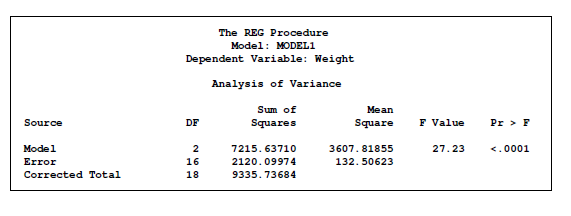
\includegraphics{images/listing}
\end{figure}
\begin{figure}[H]
\caption{LaTeX Output, default style}
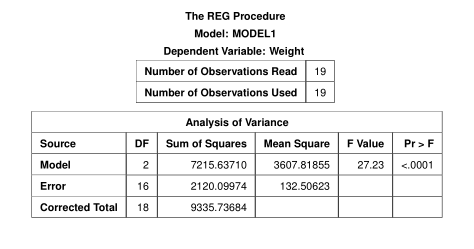
\includegraphics{images/default}
\end{figure}
\begin{figure}[H]
\caption{LaTeX Output, \texttt{statistical} style}
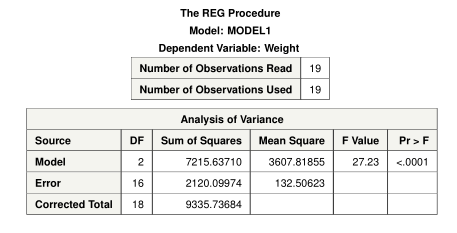
\includegraphics{images/statistical}
\end{figure}
\begin{figure}[H]
\caption{LaTeX Output, \texttt{journal} style}
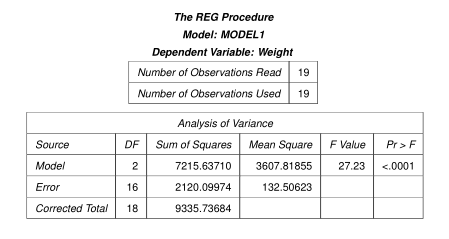
\includegraphics{images/journal}
\end{figure}
\begin{figure}[H]
\caption{LaTeX Output, \texttt{htmlblue} style}
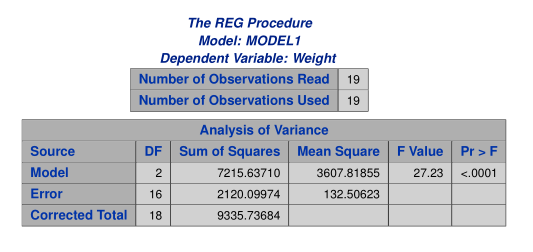
\includegraphics{images/htmlblue}
\end{figure}


\printindex
\end{document}